\documentclass[a4paper,12pt]{report}
\usepackage[margin=1in]{geometry}
\usepackage[T1]{fontenc}
\usepackage[utf8]{inputenc}
\setcounter{secnumdepth}{3}

\usepackage[long,nodayofweek]{datetime}

\usepackage{siunitx}
\usepackage[ampersand]{easylist}

% % % % % % % % % % Helpers
\usepackage{easy-todo}

% % % % % % % % % % Figure
\usepackage{graphicx}
\usepackage{wrapfig}
\graphicspath{ {Images/} }

\usepackage[backend=biber,citestyle=ieee,doi=false,isbn=false]{biblatex} 
\addbibresource{./Bibliography/Thesis.bib}

\AtEveryBibitem{\ifentrytype{misc}{}{
    \clearfield{url}
    \clearfield{urldate}
  }
}

\usepackage[nonumberlist,acronym,toc,shortcuts]{glossaries}
\robustify{\gls}% Make \gls not fragile
\loadglsentries[main]{Abbreviations}
\makeglossaries

\renewcommand*{\thefootnote}{\fnsymbol{footnote}}

\usepackage[hidelinks]{hyperref}
\usepackage[all]{hypcap}

% % % % % % % % % %Chapter Title Encoding
\usepackage{titlesec, blindtext, color}	
\definecolor{gray75}{gray}{0.75}
\newcommand{\hsp}{\hspace{10pt}}
\titleformat{\chapter}[hang]{\huge\bfseries}{\thechapter\hsp\textcolor{gray75}{|}\hsp}{0pt}{\LARGE\bfseries}

% % % % % % % % % % Symbols for footnotes


% Title Page
\title{Master Thesis Report}
\author{PrithviRaj Narendra}


\begin{document}

\maketitle

\begin{abstract}
Hello Abstract.
\end{abstract}

\tableofcontents

\printglossary[title=List of Abbreviations,type=\acronymtype]

\chapter{Introduction}

\section{General Introduction to the Domain of the Thesis}

%\todo{need more citations in this section?}
A future is envisioned where objects around us can no only communicate with us but also themselves. These \emph{smart} devices such ranging from simple key-chains and chopping boards to complex bio-implants and automobiles can sense their surroundings, communicate with humans and other objects and react to commands and external environment. There has been a lot of work on the communication protocol aspect of this scenario of \gls{iot}. This Master thesis looks into one such protocols prevalent in the low energy domain, namely \emph{\gls{ble}} and compares it with another one called \emph{802.15.4}. Also this project works with an \gls{os} developed specifically for \gls{iot} devices called \emph{Contiki}.

\gls{ble} is an addition to the Bluetooth specification to enable  development of low cost, tiny devices which can communicate wirelessly anywhere in the world while consuming ultra low power\cite{CoreSpec4.0}. Being standardized by Bluetooth \gls{sig} in 2010 with Bluetooth 4.0 version, it has been widely adopted in all the major mobile \glspl{os} and millions of devices capable of \gls{ble} communication have been sold. It has even spawned off a new category of devices called \emph{appcessories}\cite{ubiquityBeyond}, called so because these `accessories' devices are controlled from mobile `applications'. 

Contiki is a permissive open source operating system for resource constrained, networked systems developed for this \gls{iot} vision, especially for \glspl{wsn}\cite{Contiki}. Contiki's design is such that it can work with only 10 kB of \gls{ram} and 30 kB of non-volatile memory for code storage, making it suitable for even 8-bit \glspl{mcu} running at few MHz. Contiki because its free, support to a wide variety of hardware platforms and the mature status of its development, it is used in wide range of projects ranging from commercial thermostats to research on badger behavior. 

802.15.4 based transceivers form the basis for communication in majority of projects running on Contiki. 802.15.4 is a physical and \gls{mac} layer specification for low data rate wireless networks, defined in 2003\cite{IEEE802154}. Contiki's networking stack does not use the standard 802.15.4 \gls{mac}, but in-house developed \gls{mac} layers such as ContikiMAC, Null-RDC and MiCMAC. This layer plays a critical role in determining the power consumption, data rate, latency and resistance to external interference and error in communication. 


%What is Contiki \gls{os}? Why was it and who/where is it being used? Explain the amount of R\&D done in terms of communication protocols based on 802.15.4 .


\section{Problem Definition}

Contiki is providing features to facilitate and ease development of \gls{iot} applications such as Coffee flash file system, \gls{mcu} emulation (MSP430 and AVR based), network simulator (Cooja), power usage estimator (Energest), wide range of hardware platforms and a host of networking protocols including full standard IP stack, 6LowPAN, RPL and CoAP. Adding support for \gls{ble} support for Contiki would go a long way in increasing the support Contiki offers for \gls{iot} applications, now that \gls{ble} has been so successful with its adoption in mobile devices. This make even greater sense considering the fact that Bluetooth core specification 4.1 lays the ground framework for inclusion of IPv6 in \gls{ble}\cite{4.0to4.1} and Internet Engineering Task Force (IETF)  has a working draft on transmission of IPv6 packets over \gls{ble}\cite{ieftIPv6Draft}.

For product developers, researchers and hobbyists alike, a comparison of 802.15.4 and \gls{ble}'s link layer would quite helpful for understanding their characteristics, knowing their pros \& cons and finally identifying the suitable applications for these protocols. This would be especially useful in the context of being used in Contiki with the use of Contiki's \gls{mac} layers such as ContikiMAC and Null-RDC. 

%Need for \gls{ble} in Contiki as a platform for \gls{iot}. To understand the characteristics of \gls{ble} and 802.15.4 so that we can identify the applications suitable for these protocols.

\section{Problem Context}

This Master thesis was done in the Networked Embedded Systems (NES) group of Swedish Institute of Computer Science (SICS) to yield greater insight in the \gls{ble} protocol and provide a base for further research in this topic.

\section{Goals}

This thesis project aims to start the process of including \gls{ble} support in Contiki by including a \gls{ble} based platform in the list of hardware platforms supported by Contiki. This is done by studying the BLE standard, comparing and choosing a BLE based hardware platform to Contiki can be ported to, followed by the actual porting and finally using the Contiki port. 

The comparison of Contiki's 802.15.4 based \gls{mac} layers with \gls{ble} link layer starts by defining the performance metrics, namely data rate, latency, reliability and energy consumption. Test cases are then designed to compare these metrics for the two protocols. To study the effect of external interference, these test cases include scenarios with and without external WiFi traffic. This comparison of the two protocols is concluded by summarizing the data acquired, analyzing this information and comparing it with the information from the existing literature in this topic.

%Evaluate and compare the performance of physical and link layer on
%BLE and 802.15.4 based platforms
%Compare data rate, latency, energy consumption and reliability
%(packet reception ratio - PRR)
%Compare with different energy saving mechanisms in 802.15.4
%platform i.e. Out of the box MAC, ContikiMAC, NullMAC and
%multichannel MAC
%Evaluate in multichannel environment with interference

%To choose and integrate a \gls{ble} hardware platform with Contiki. To compare \gls{ble} and 802 in various performance criteria of data-rate, latency, reliability and energy consumption in environments with and without external interference.

\section{Outline of the report}

This report starts off by providing the necessary background information required to follow this report in chapter \ref{2Back}. Chapter \ref{3Method} provides an overview of the research process and methodology employed in this thesis. The existing literature available in this research topic is explored in chapter \ref{4LitStudy}. The porting of Contiki to a new platform, specifically the nrf51822 based platform is described in chapter \ref{5bleContiki}. The objectives of this research and the test cases designed to reach these objectives are detailed in chapter \ref{6Testing}. Chapter \ref{7ResultsAnalysis} showcases the data acquired from conducting these tests in graphical forms, analyses this information and draws results. Chapter \ref{8OtherContri} briefly describes the additional work done in this thesis, not entirely in-line with the research process of this thesis. This report finishes off with providing the conclusions and recommends the prospective work that can be done in the direction of this research.

\listoftodos

\chapter[Background]{Background\footnote{Contains text \& images from the author's Minor Thesis `Business Ideation for \gls{ble}', derived from this thesis' work}} \label{2Back}

This chapter aims at providing a succinct background necessary to understanding the rest of the thesis report. Readers are directed to the references for a comprehensive overview. Section \ref{OverviewBLE} provides an overview of the BLE technology required for following this document. Description of Contiki \gls{os} and literature involving the process of porting of Contiki \gls{os} to a hardware platform are presented in section \ref{OverviewContiki}. This chapter ends with presenting the aspects related to the 802.15.4 protocol utilized in this project.


\section{Overview of \acrlong{ble}} \label{OverviewBLE}

\acrfull{ble} is a relatively new low power standard incorporated in Bluetooth Core Specification Version 4.0 released by Bluetooth \gls{sig} in 2010\cite{CoreSpec4.0}. This wireless personal area network is marketed as Bluetooth Smart the Bluetooth \gls{sig}. Devices containing only BLE hardware are \emph{single mode} devices, whereas devices containing both classic Bluetooth and BLE are known as \emph{dual mode} devices.   

\gls{ble} was designed by Bluetooth \gls{sig} from the ground up, which helped it achieve certain design goals. These design goals for this wireless personal area network were \emph{low cost, worldwide operation, short range, robustness} and \emph{low power}\cite{Heydon2012}. One most important differentiating factors that has made BLE so successful is the standardization by Bluetooth SIG, facilitating its inclusion in consumer devices and enabling communication across different vendors. In 2013, over 85\% consumer electronic devices supported BLE, making it the de facto standard for low power wireless communication in these devices\cite{Martin2014}. BLE is adopted for various control, notification and monitoring applications, especially in the healthcare, fitness, security and home entertainment industry. 

%\subsection{Design objectives of \gls{ble}}
%
%\paragraph{Low Power} \gls{ble} aims to use a tiny batteries such as button cell to keep a device operating for months to years. To achieve this goal, \gls{ble} was optimized to communicate small amounts of data, such as the states of devices. Also \gls{ble} is optimized to have lower peak power requirements, which allows use of button cells to be used with \gls{ble} devices.
%\paragraph{Worldwide Operation}
%For a technology to be adopted, it is important that there is uniform conformity to the regulations around the world. The 2.4 \si{\GHz} \gls{ism} radio band is the only one available license free worldwide. The technology to develop wireless devices in this band is mature making it the suitable radio band for \gls{ble}.
%\paragraph{Short Range}
%\gls{ble} was designed to be for personal area network like Classic Bluetooth, which means that it is not a network to work with a cellular base station network. This design criterion goes hand in hand with \emph{low power}.
%\paragraph{Low Cost} Lower power requirements mean that the batteries in \gls{ble} devices need to smaller and have to be replaced less frequently, both resulting in a reduction of cost for both the manufacturer and the customer. The use of the \gls{ism} band for communication levels removes the licensing entry barrier for start-ups to develop \gls{ble} devices. \gls{ble} embraces simplicity in its pursuit to lower the cost. \gls{ble} supports only single-hop communication in a star network, which reduces the memory and processor requirement for supporting the protocol. Simplicity was the key factor for the choosing of \gls{gfsk} as the modulation scheme for \gls{ble} to result in low cost, simple implementation of the radio in the \glspl{ic} for \gls{ble}. 
%\paragraph{Robustness} The 2.4~\si{\GHz} space is crowded with devices communicating with various standards as well as spurious noise making the robustness a key criteria in developing \gls{ble} standard. \gls{ble} uses a multi-channel hopping mechanism called \gls{afh} to detect, avoid and recover from interference. In addition to \gls{afh}, \gls{ble} uses \gls{crc} to detect and recover from bit-errors due to background noise.

\subsection[\gls{ble} Network Architecture]{\gls{ble} Network Architecture\cite{BLE101}}

\begin{table}[htbp]
\begin{center}
\vspace{-10pt}
\setlength{\extrarowheight}{1.5pt}
\begin{tabular}{|m{2.5cm}|m{1.2cm}|m{11.4cm}|}
\hline
\multicolumn{ 2}{|c|}{\textbf{State}} & \textbf{State Description} \\ \hline
\multicolumn{ 2}{|c|}{Standby} & Does not transmit or receive packets, usually sleeping \\ \hline
\multicolumn{ 2}{|c|}{Advertising} & Broadcasts advertisement packets in  advertising channels \\ \hline
\multicolumn{ 2}{|c|}{Scanning} & Looks for advertisement packets, across advertising channels \\ \hline
\multicolumn{ 2}{|c|}{Initiating} & Initiates connection to advertiser to get Master role \\ \hline
\multicolumn{ 1}{|m{2.0cm}|}{\hspace{42pt} \mbox{Connection}} & Master & Communicates with device(s) in the \emph{slave} role, defines configuration of the connection \\ \cline{ 2- 3}
\multicolumn{ 1}{|l|}{} & Slave & Communicates with a single device in \emph{master} role \\ \hline
\end{tabular}
\end{center}
\vspace{-12pt}
\caption{Possible states of a BLE device}
\vspace{-6pt}
\label{tbl:BLEstates}
\end{table}

Table \ref{tbl:BLEstates} shows the possible states of a BLE device and figure \ref{fig:Roles} illustrates the ways in which these states can change. The standby role is universally supported across all BLE devices and the other roles are present in device according to their configuration. For example, a device with only a radio transmitter can alternate between the advertising and standby state, usually called an \emph{advertiser}. Similarly a \emph{scanner} can just receive BLE packets.

\begin{wrapfigure}{r}{0.55\textwidth}
\centering
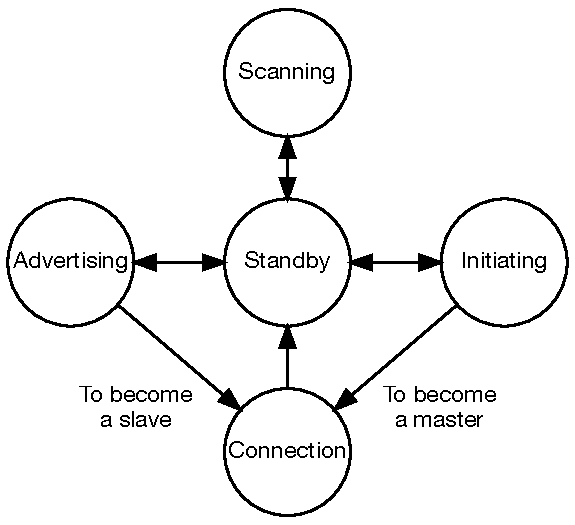
\includegraphics{Roles.pdf}
\caption{State diagram of BLE states}
\label{fig:Roles}
\vspace{-10pt}
\end{wrapfigure}

A connection can be formed between two BLE devices, with the master node reaching from the initiating state and the slave node from the advertising state. This master and slave roles follows an asymmetric design philosophy. A slave is a simple device that can be connected with at most one master at a time and are usually single purpose devices. A master on the other hand is a more complex device which is responsible for coordinating the connections and activities of all the slaves connected to it. A master is usually a multi-purpose device such as a mobile phone, tablet or a laptop. A master connected with multiple slaves employs a star topology. The slaves cannot directly communicate with each other. An example of a BLE network is shown in figure \ref{fig:TopoBLE}. Here a master can be seen connected to multiple slaves. The bidirectional continuous lines show data communicated in both directions when in a connection. The dashed lines show the data from the advertisements being sent broadcast. A master or slave can be an advertiser simultaneously as seen in the figure \ref{fig:TopoBLE}.  

\begin{figure}[h]
\centering
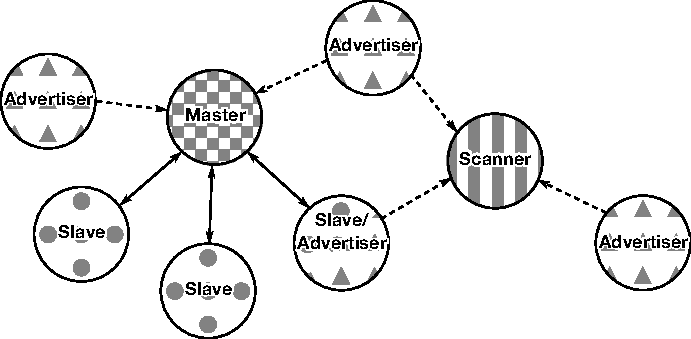
\includegraphics{TopologyBLE.pdf}
\caption{An example of BLE topology}
\label{fig:TopoBLE}
\end{figure}

%\begin{figure}[h] %{r}{0.51\textwidth}
%%\vspace{-15pt}
%  \begin{center}
%	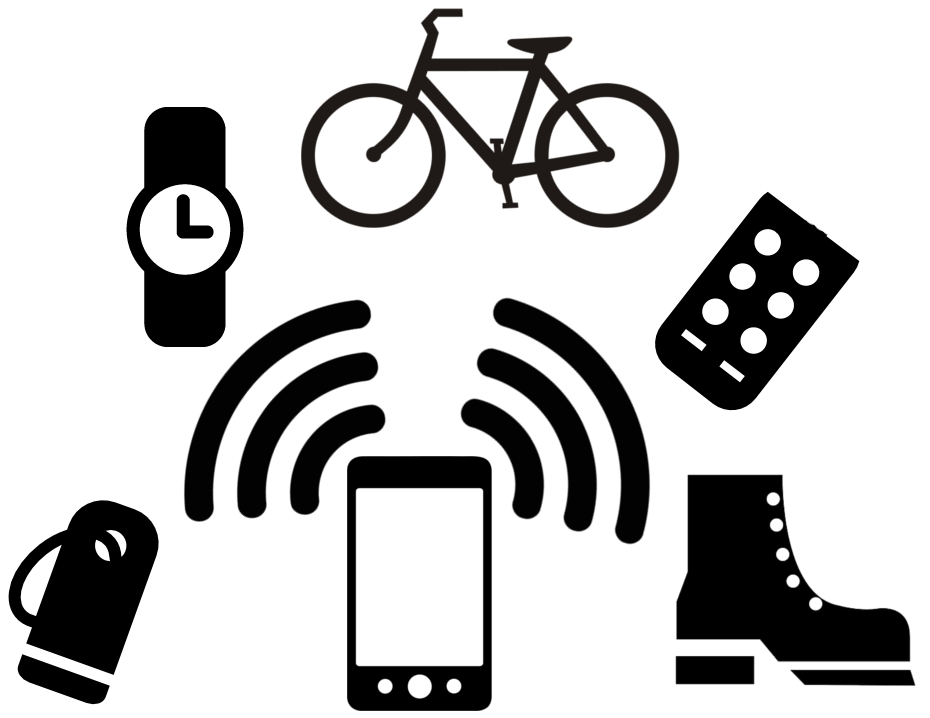
\includegraphics[width=0.49\textwidth]{devicesBLE}
%  \end{center}
%\caption{Typical BLE network}
%%\vspace{-10pt}
%\label{devicesBLE}
%\end{figure}

\section[\gls{ble} stack overview]{\gls{ble} stack overview\cite{Heydon2012}}

To implement the BLE network described in the previous section, the BLE stack used is as shown in figure \ref{fig:StackBLE}. The BLE stack is split into a host section and a controller section. The controller part takes care of the actual interaction with the radio and enforcing the timing requirements. The controller part is implemented in the \gls{ic} where the radio is located, usually the \gls{soc} or the discrete transceiver. On the other hand, the host contains the software required for handling the various kinds of BLE packets. This separation of host and controller allows mixing and matching of these parts from different sources. The communication between the host and controller is done through the Host Controller Interface. The rest of this section explains the different layers briefly, with emphasis on the parts used in this thesis.

%\begin{figure}[h]
%\begin{center}
%\setlength{\extrarowheight}{1.5pt}
%\begin{tabular}{|c||c|c|}
%\cline{2-3}
%\multicolumn{1}{c|}{} &  \multicolumn{ 2}{c|}{Applications} \\ \hline
%\multicolumn{ 1}{|c||}{} & \multicolumn{ 2}{c|}{Generic Access Profile} \\ \cline{ 2- 3}
%\multicolumn{ 1}{|c||}{Host} & \multicolumn{ 2}{c|}{Generic Attribute Profile} \\ \cline{ 2- 3}
%\multicolumn{ 1}{|l||}{} & \multicolumn{1}{c|}{Attribute Protocol} & \multicolumn{1}{c|}{Security Manager} \\ \cline{ 2- 3}
%\multicolumn{ 1}{|l||}{} & \multicolumn{ 2}{c|}{Logic Link Control and Adaptation Protocol} \\ \hline \cline{2-3}
%\multicolumn{1}{c|}{} & \multicolumn{ 2}{c|}{Host Control Interface} \\ \cline{2-3} \hline
%\multicolumn{ 1}{|c||}{Controller} & \multicolumn{1}{c|}{Link Layer} & \multicolumn{1}{c|}{Direct Test Mode} \\ \cline{ 2- 3}
%\multicolumn{ 1}{|c||}{} & \multicolumn{ 2}{c|}{Physical Layer} \\ \hline
%\multicolumn{ 1}{c}{} & \multicolumn{1}{m{4cm}}{} & \multicolumn{1}{m{4cm}}{} \\ 
%\end{tabular}
%\end{center}
%\vspace{-30pt}
%\caption{BLE Stack}
%\label{fig:StackBLE}
%\end{figure}

\begin{figure}[h]
\begin{center}
\setlength{\extrarowheight}{1.5pt}
\begin{tabular}{|c||c|c|}
\cline{2-3}
\multicolumn{1}{c|}{} &  \multicolumn{ 2}{c|}{Applications} \\ \hline
\multirow{4}{*}{Host} & \multicolumn{ 2}{c|}{Generic Access Profile} \\ \cline{ 2- 3}
 & \multicolumn{ 2}{c|}{Generic Attribute Profile} \\ \cline{ 2- 3}
 & \multicolumn{1}{c|}{Attribute Protocol} & \multicolumn{1}{c|}{Security Manager} \\ \cline{ 2- 3}
 & \multicolumn{ 2}{c|}{Logic Link Control and Adaptation Protocol} \\ \hline 
\multicolumn{1}{c|}{} & \multicolumn{ 2}{c|}{Host Control Interface} \\ \hline
\multirow{2}{*}{Controller} & \multicolumn{1}{c|}{Link Layer} & \multicolumn{1}{c|}{Direct Test Mode} \\ \cline{ 2- 3}
 & \multicolumn{ 2}{c|}{Physical Layer} \\ \hline
\multicolumn{ 1}{c}{} & \multicolumn{1}{m{4cm}}{} & \multicolumn{1}{m{4cm}}{} \\ 
\end{tabular}
\end{center}
\vspace{-30pt}
\caption{BLE Stack}
\label{fig:StackBLE}
\vspace{-10pt}
\end{figure}

\paragraph{Physical layer}
This is layer with the actual task of sending and receiving electromagnetic signals with a 2.4 GHz \gls{ism} radio. The modulation scheme used is \gls{gfsk}. The bit rate used is 1 Mbps. There are 40 channels over which BLE operates, each 2 MHz apart from each other. In these there are 3 advertisement channels for sending advertisement packets. These are spread over the \gls{ism} band, located where overlapping with WiFi signals does not occur. The rest of the channels are used for communicating data when in connection mode.

\paragraph{Link layer}
The link layer is responsible for advertising and scanning when unconnected, along with creating and maintaining connections. The error detection and encryption are also taken care by this layer. 

The process of connection establishment happens when a advertising device gets a `connection request' packet, which contains the specifications of all the parameters required to maintain the connection. The advertising device becomes the slave and the device which sent the connection request packet becomes the master. The three parameters that are primarily dealt with in this thesis are as follows.
\begin{easylist}[itemize]
& \textbf{Connection Interval} \hspace{5pt} After a BLE connection is established, the master device must always send a packet to the slave periodically with a time period specified as connection interval. If there is nothing to communicate, an empty packet is sent. These connection \emph{events} provide an opportunity for the slave to communicate with the master. 

& \textbf{Slave Latency} \hspace{5pt} The maximum number of connection events that a slave can choose not to respond to the master. This is intended to save power on the slave while also providing an opportunity to communicate with the master if necessary. If slave latency is zero, the slave must respond with an empty packet in every connection event even it does not have any reason to communicate.

& \textbf{Hop Increment} \hspace{5pt} BLE employs a frequency hopping mechanism to spread the communication over the entire 2.4 GHz band. This is achieved by the master initiating communication in each connection event in a different data channel, among the 37 data channels. The hopping of the master is synchronized with the slave with the following algorithm.

\hspace{160pt}$f_{n+1}=(f_n + hop) \hspace{2pt} \% \hspace{2pt} 37$ 

Where, `\%' denotes the modulus operation, $f_{n+1}$ is the next channel that will be used, $f_n$ is the current channel used and $hop$ is the hop increment parameter sent when establishing a connection.

& \textbf{Channel Map} \hspace{5pt} This parameter specifies the channels utilized by the frequency hopping algorithm. Usually, the entire channel map of 37 data channels is utilized. If some channels are detected to be unusable because of external interference, the channel map can be updated to utilize only a subset which is free of interference. This mechanism is called \gls{afh}, where the channels used for communication is adapted according to the external conditions, leading to increase in robustness of communication.
\end{easylist}

Error detection in BLE communication is performed by utilizing 24 bit \gls{crc} in every packet. A simple acknowledgment scheme is used to request retransmission in case an error is detected or packet reception does not happen. This uses two bits called `\gls{sn}' and `\gls{nesn}'. When a device gets a packet with a particular \gls{nesn},  it must use that as \gls{sn} when it transmits a packet. In case a packet is missed, the device does not know \gls{nesn} and uses the old \gls{sn} in its transmitted packet, thus indicating that it did not receive the last packet. This is better illustrated in figure \ref{fig:SeqNum}. When the slave's packet is lost, the master uses the previous \gls{sn}, thus indicating retransmission. After that the \gls{sn} follows \gls{nesn}.

\begin{figure}[h]
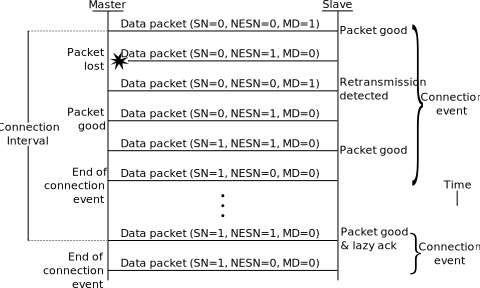
\includegraphics[width=\textwidth]{SeqNum}
\caption{Illustration of working of BLE link layer's \gls{sn}, \gls{nesn} and \acrshort{md}}
\label{fig:SeqNum}
\end{figure}
 
Another important parameter used in maintaining BLE connection is the `\gls{md}' bit. The \gls{md} bit indicates if a device has more data to send, so that more packets can be exchanged in a connection event. In figure \ref{fig:SeqNum}, the master has \gls{md} set to one while slave has it set to zero, indicating that the master has more data to send. In this case the master and slave exchange two packets in a connection event until both master and slave have \gls{md} as zero. In the second connection event, both master and slave have \gls{md} as zero, causing the connection event to end after exchange of one packet. \gls{md} bit allows communication of multiple packets in a connection interval when there is large amount of data to be communicated, thus increasing the throughput.

\paragraph{\gls{l2cap}} This layer is responsible for multiplexing data from different logical channels in BLE, although in Bluetooth 4.0 only three fixed channels are used. 

\paragraph{Security Manager} This layer is used for pairing BLE devices, which is a form of authenticating the other device. Typically this is followed by encryption key distribution.

\paragraph{\gls{att}} This layer defines the \emph{Client-Server} architecture used by BLE to communicate data. A server is where data is held in a database and a client is one which gets the data from a server. All data stored in BLE devices as \emph{Attributes}, which is data organized in a specific format containing a label and address. Thus, a client can requests and gets a specific attribute from a server's database. Client or server configuration is independent of the role in link layer. A master or slave device can have \emph{both} a client and a server.

Attributes can be accessed from the attribute database in six ways as listed below.

\begin{easylist}[itemize]
& Find Requests: Client can find the attributes present in server's database.
& Read Request: Clients requests to get an attribute in server, to which the server responds with the requested attribute.
& Write Request: Client writes to an attribute in server with acknowledgment back.
& Write Command: Client writes to an attribute in server without acknowledgment back.
& Notification: Unprompted by the client, server sends an attribute to a client, to which the client does not acknowledge.
& Indication: Unprompted by the client, server sends an attribute to a client, to which the client acknowledges.
\end{easylist}

\paragraph{\gls{gatt}}
This layer organizes the attributes in a hierarchical manner, so that similar attributes can be encapsulated together.

\paragraph{\gls{gap}}
This layer defines how BLE devices discover, connect and present useful information to the users and each other. A device having peripheral \gls{gap} role advertises and then connects to become a slave at link layer. A \gls{gap} central device initiates connection to a peripheral and becomes a master at link layer once connected.

\section[Overview of Contiki \gls{os}]{Overview of Contiki \gls{os}} \label{OverviewContiki}

Contiki \gls{os} is a lightweight, mature and open source operating systems with extensive networking stack for low cost and low power systems\cite{Contiki}. In this document `Contiki' and `Contiki \gls{os}' have been used interchangeably and mean the same thing. Contiki's networking capabilities include the complete IP stack (IPv4, IPv6, UDP, TCP, HTTP) and the recent \gls{ietf} standardized protocols for IPv6 networking such as RPL multihop routing protocol, 6LowPAN and CoAP RESTful application layer protocol. For the event driven scheduler that Contiki uses, a mechanism called \emph{Protothreads} is used. This results in low memory foot-print and nice flow control in code development. Another tool developed to ease development using Contiki, especially in large distributed systems is \emph{Cooja}. Cooja is a network simulator that has the capability of simulating large scale network on emulated hardware units with fine grained control. Cooja was used in this thesis also to verify designed before actually deploying them. Low power \glspl{wsn} is the typical application scenario of devices running on Contiki, although Contiki has been used in a wide variety of projects.



\subsection{Porting the Contiki to a New Platform} \label{2Porting}
Contiki \gls{os} has been ported to an increasing number of hardware platforms \cite{contikiHw}. Since Contiki is an open-source BSD Clause-3 licensed project, there are many projects in various hardware platforms based on a fork from the Contiki repository.

These hardware platforms' processors range across a spectrum of 8-bit (8051 and AVR), 16-bit (MSP430) to 32-bit (ARM Cortex-M, PIC32). Contiki has support for 802.15.4 based wireless communication with various external transceivers and \glspl{soc} with radio transceiver built in the same \gls{ic} as the \gls{mcu}. Various common features of many platforms such as \glspl{led}, buttons and serial port have modules in Contiki for common \gls{api} across platforms.

In \cite{Oikonomou2011} the authors describe Contiki's port to a CC2430 based platform manufactured by Sensinode Ltd. CC2430 is an enhanced Intel 8051 processor based \gls{soc} having 802.15.4 physical layer compatible radio transceiver. The authors fully debugged the port which had of a code footprint of about 100 kB, varying based on the compiler mode and the features enabled. Many new features were added to the port including support for \gls{adc} unit, all the sensor available on the platform (accelerometer, light sensor, voltage and temperature sensors), watchdog timer and the general purpose buttons. Because of the limited stack availability of 233 bytes, many optimizations such as moving variables to external \gls{ram} memory space and re-writing the radio driver for CC2430 to prevent stack from overflowing.

Contiki was ported to two new platforms, namely MicaZ and TelosB in a Bachelor thesis \cite{stan2007porting}. TelosB, similar to the TMote-Sky platform, consists of a 8MHz 16-bit MSP430 \gls{mcu}, a CC2400 transceiver with 802.15.4 \gls{phy} and a host of sensors to measure light, temperature and humidity. The port to TelosB was done by changing the port to the fully supported TMote-Sky platform. MicaZ platform consisted of a 8-bit Atmel ATMega128L \gls{mcu} and a CC2400 transceiver. MicaZ platform needed rewriting of the code for processor abstraction so that the high level Contiki \glspl{api} could work.

Contiki has been ported into platform based on a ARM Cortex M3 processor to create a device wired with Ethernet to connected to the Internet \cite{Wilde2013a}. Ethernet based networking with the libraries present in Contiki was developed in this project to demonstrate as a proof of concept. There are many unofficial ports of Contiki to various hardware platforms.

\section{Overview of 802.15.4} \label{Overview15.4}
Mention that in this thesis the Contiki specific implementations of the 802.15.4 layers will be tested.

\subsection{Physical layer}
802.15.4 also uses the 2.4 GHz \gls{ism} band for communication, with this spectrum divided into 16 channels numbered from 11 to 26. The bit rate used for this standard is 250 kbps.

\subsection{\gls{mac} layer}

The link layer of 802.15.4 consists of \gls{mac} layer on top of a \gls{rdc} layer. For the RDC layer the Null-RDC and ContikiMAC driver will be tested in each of the test with \gls{csma} as the \gls{mac} layer. In case of Contiki-MAC the receiving node switches on periodically to sense if there are any packets that need to be received. The default time of this period is 125 ms. In case of null-RDC the radio receiver is never switched off, as the name suggests.


\subsubsection{\gls{rdc} layer}
\subsubsection{\gls{csma}}



\chapter{Methodology}

\section{Research Process}

Figure \ref{RePrSteps} shows tasks performed in this thesis as boxes of the flow-chart and the steps of the research process on the left. The thesis report is also organized in this manner.

\begin{figure}[h]
\centering
\def\svgwidth{0.93\columnwidth}
\input{./Images/RePR.pdf_tex}
\vspace{-10pt}
\caption{Thesis' tasks and steps in the research process}
\label{RePrSteps}
\end{figure}

\section{Research Method}

In this experimental research large amount of data was generated to compare the two protocols mentioned, hence utilizing quantitative research method. The approach followed was deductive as the experiment started by defining the metric to measure, then designing the test to perform and finally deducting the conclusions based on the collected data from the tests.

The data collected was condensed with descriptive statistics and graphical representation was used to showcase this information. Univariate analysis  of the various metrics of the two protocols was done to compare the two protocols from these graphical representation.
\chapter{Literature Study} \label{4LitStudy}

This chapter provides a brief overview of the related work being done in the research community. Performance evaluation of \gls{ble}, 802.15.4 and their comparison are presented in section \ref{4ble}, \ref{4802} and \ref{4ble802} respectively. The comparison of the existing literature with the results produced in this thesis is explained in section \ref{7Eval} in the `Results and Analysis' chapter.

\section{Evaluating the Performance of \texorpdfstring{\gls{ble}}{BLE}} \label{4ble}
In a paper  \cite{Gomez2012} providing an overview and evaluation of \gls{ble}, its various parameters such as energy consumption, latency, maximum piconet size and throughput have been evaluated. Theoretical calculations were done to predict the lifetime of a \gls{ble} slave device running of a 230 mAh coin cell battery for different values of connection interval and slave latency. The average current consumption of a TI CC2540 \gls{ble} platform was plotted for the entire range of connection interval keeping the slave latency as zero. The estimate of the lifetime was also done with respect to various \gls{ber}. A latency measurement also has been done in this paper, where it measures the time to send a notification packet and receive the `no more data' acknowledgment packet from the receiver in the link-layer. This interaction happening in the same connection event was measured as 676.7 \si{\micro \second}.

The same experimental setup  \cite{Gomez2012} shows the maximum throughput between two CC2540 devices as 58.48 kbps considering a payload of 20 bytes. This is attributed to the fact that in each connection event with an interval of 7.5 ms four packets are not transmitted as in an ideal case. An analytical model of the throughput  \cite{Gomez2011} has been developed for different \gls{ber} and connection interval. Simulation results validate this model developed. This model show that the maximum throughput in case the \gls{ber} is zero is 236.7 kbps, independent of the connection interval. An assumption made in this paper is that the master and slave device do not have any limit on the number of packets communicated in a connection interval. 

The energy consumption for an advertiser and scanner is modeled for the activity of the scanner discovering the advertiser  \cite{liu2012energy}. The current consumption for each phase of advertisement and scanning is measured. Using this information a model of the energy consumption is developed taking into account the advertising and scanning interval. The model developed is compared with experiments and validated. 

The current consumption in the different phases of a connection event, namely waking up, pre-processing, the transmission-reception cycles and the post-processing is measured  \cite{Mackensen2012} to estimate the lifetime. The same article found the throughput achievable for a payload of 20 bytes as around 40 kbps. A recent journal article  \cite{Kindt2014} develops a precise model of the energy consumption of \gls{ble} devices. A payload (20 bytes) throughput of 102 kbps is achieved in this paper, consistent with the manufacturer's claims  \cite{MikkoSavolainen}. The model developed is  unique in the sense that it is the first one which encompasses all the modes of operation, all the relevant parameters and their possible values. The model is based upon the actual measured duration of various parameters and measured current in various phases of operation. This leads to a model which at most has 6\% variation from actual measurement. The code base for the model is available so that it can be ported to the system being evaluated.

Based on the model developed and evaluated, a set of guidelines are provided for developers of \gls{ble} system to reduce energy consumption  \cite{Kindt2014}. In the unconnected mode, the scanner is recommended to be continuously scanning in case the advertisers is expected to be found soon. In case of where a lot of time is spent scanning idly, the parameters of advertising interval and duty cycle of the scanner can be tweaked to minimize both the energy consumption and latency of discovery. In the connected mode, the recommendation is to completely fill the payload as possible and communicate as much data as possible within a connection event. In both modes, it was noted that although reducing the transmission power appropriate to the the distance transmitted helped in reducing energy consumption, it was not as significant as the other factors.

The interference caused by WiFi over \gls{ble} advertisement packets and vice versa has been evaluated \cite{Wyffels}. This paper tests two cases, one where a BLE advertising channel overlaps with a WiFi channel and one where it does not. In the case where the there was no overlap of the two wireless protocols, there was negligible influence of each other. Increasing the advertising devices from 1 to 21 increased the \gls{crc} error and decreased the packets sniffed by the scanner per device from 40 to 22 because of the collision of the advertising packets. In case where there was overlap of the WiFi and BLE channels, there the WiFi throughput decreased to 50\% as the number of advertisers increased from 1 to 21. The scanner experience a greater number of \gls{crc} errors, thereby decreasing the number of packets sniffed per device, decreasing to almost 50\% of the previous case.

\section{Evaluating the Performance of 802.15.4} \label{4802}

As mentioned in section \ref{Overview15.4}, this thesis will not use the standard 802.15.4 standard MAC layer, only the 802.15.4 physical layer. The MAC layers used with 802.15.4 physical layer are ContikiMAC and Null-RDC. This is because of the amount of activity in the research community with these layers as compared to the standard 802.15.4 MAC layer. This section will briefly explain the research done to evaluate the performance of ContikiMAC, Null-RDC and other \gls{mac}. There are few research articles which compare the performance of 802.15.4 for point to point networks as multi-hop networks are preferred for analysis.

ContikiMAC is detailed in a technical report  \cite{Dunkels2011} which also evaluates its performance with few benchmarks. The radio on time and current consumed for different types of reception and transmission have been represented graphically. The performance of a 20 node network has been benchmarked with simulation in Cooja Network Simulator. The \gls{rdc} for a data collection network of with path loss using ContikiMAC was less than 2\% for up to about 25 Hz channel check rate, with the least being less than 1\%. The optimizations of phase lock and fast-sleep can be seen to reduce the \gls{rdc} significantly, especially when there is path loss.

The maximum throughput for packet transmission through a  network of 139 nodes was evaluated with a new protocol called P\textsuperscript{3}  \cite{Doddavenkatappa2014}. The goodput, which is the application level throughput, was significantly improved compared to the existing solution. It ranged from 142.9 kbps to 199.7 kbps depending on the route used in the network, with an average of 175.2 kbps.

Latency, power consumption and reliability of point to point communication using 802.15.4 has been evaluated for different \gls{mac} layers \cite{Uwase2014}. The latency for ContikiMAC and Null-RDC for a round trip measurement was measured as 103 ms and 5 ms respectively. ContikiMAC increases the latency by an order of 20 times while consuming 13 timess lesser power than Null-RDC. The packet delivery ratio of Null-RDC was measured as 100\% while ContikiMAC had a reliability of 90\%.

The authors in \cite{Duquennoy2011} present a mechanism to allow high-throughput data transfer in a lossy environment while also conserving power. This generic packet forwarding technique called \emph{burst forwarding} and is implemented with ContikiMAC. This mechanism enables throughput of 5.8 kBps for bulk transfer over eight hops from transmitter to receiver. 

% \cite{Michel2014} Mathieu Michel and Bruno Quoitin. “Technical Report : ContikiMAC vs X-MAC performance analysis”. In: arXiv preprint arXiv:1404.3589 (Apr. 2014). arXiv: 1404.3589.

% \cite{Uwase2014} M.-P. Uwase, M. Bezunartea, T.L. Nguyen, et al. “Experimental evaluation of message latency and power usage in WSNs”. In: 2014 IEEE International Black Sea Conference on Communications and Networking (BlackSeaCom). IEEE, May 2014,


\section{Comparison of \texorpdfstring{\gls{ble}}{BLE} and 802.15.4} \label{4ble802}

\gls{ble} is relatively new protocol compared to 802.15.4, due to which there are few studies conducted comparing the two low power wireless protocols. The energy consumption of \gls{ble} and 802.15.4 was compared in terms of the amount of payload can be communicated per Joule of energy i.e. the energy utility measured with unit kByte/J  \cite{Siekkinen2012}. It was found that for \gls{ble} the energy utility was independent of the throughput and depended on the number of packets communicated per connection event. The energy utility varied from around 325 to 525 kByte/J when the packets per connection event rose from one to four respectively. In case of 802.15.4, the energy utility did depend on the throughput. Until 1 kBps the energy utility increased with respect to the throughput, then plateaued at 300 kByte/J. 

In the same paper  \cite{Siekkinen2012} the energy utility of both \gls{ble} and 802.15.4 is measured when transmitting a payload over the link layer and when transmitting payload with \gls{6lowpan} with the application payload (up to 150 Bytes) as a factor. Both increase in a step-wise manner because of the maximum payload capacity in both protocols with \gls{ble} having larger number of step because of the lesser payload capacity of 27 byte at the link layer. The overheads of the different \gls{6lowpan} frames can also be seen in both the protocols. 

The effect of interference caused by \gls{udp} packets sent over WiFi on the reception of packets is also considered for the two protocols  \cite{Siekkinen2012}. It should be noted that the test build did not support \gls{afh} to avoid interference, so the authors tested only the non-connected mode for \gls{ble}. In that case, up to 1 m the interference resulted in only 5 to 20\% of the packets being received successfully, depending on the overlap of the interfering WiFi channel over the advertising \gls{ble} channel. 1.5 m and above the WiFi interference affected the communication little. In case of 802.15.4, the WiFi interference closer than 0.5 m resulted in only 35\% of the packets being communicated. At a distance of 1 m and above, the interference had negligible effect on the packets being communicated.

Another journal article  \cite{Mikhaylov2013} compares \gls{ble}, 802.15.4 and another wireless protocol SimpliciTI over various criteria of throughput (theoretical and experimental), minimum turnaround time, energy consumption of the transceivers and the memory resources required for the stack of these protocols. Minimum turnaround time here is the time required for requesting data and receiving it. SimpliciTI is an flexible open-source low-power proprietary radio protocol developed by TI for their wireless products, compatible with 802.15.4 transceivers. Similar to  \cite{Gomez2011}, a the calculation of the maximum throughput for \gls{ble} provided a value greater than 300 kbps, now at the link layer. Since SimpliciTI does not have rigid specification, its parameters can be tweaked for the maximum throughput to be calculated as 350 kbps. 802.15.4's maximum throughput was calculated to be between 150 and 200 kbps. The experimental evaluation of the throughput for SimpliciTI and 802.15.4 peaked at about 160 kbps and 145 kbps respectively accounting to the pre-processing operations and CCA inc case of 802.15.4. In case of \gls{ble}, the stack allowed different number of packets per connection event based on the link layer payload size. This resulted in a the throughput increasing irregularly with the payload, peaking at 122.6 kbps.

The minimum turnaround time measured for \gls{ble} was estimated to be below 1 ms since the reply was expected after the \gls{ifs} in the same connection event. Experiments show that this is actually 7.6 ms. This is consistent with the minimum connection interval of 7.5 ms after which the reply is received in the next connection event. The minimum turnaround time was estimated as 1.92 to 10.08 ms and 0.7 to 5 ms for 802.15.4 and SimpliciTI respectively based on the mode of operation. The measured value was between 1.5 and 3 ms higher than the estimated value for both 802.15.4 and SimpliciTI. The energy consumption for the three protocols were measure per transmission and per byte transmitted. It was found that \gls{ble} transceiver consumed 2 to 7 times lower energy than the other two transceivers depending on the mode of operation.

One more article compare the energy consumption of \gls{ble}, ZigBee and ANT wireless protocols for a low duty cycle application sending few bytes of data periodically   \cite{Dementyev2013}. Standardized in 2003, ZigBee is a wireless, low cost, low power, mesh networking standard  \cite{ZigbeeAkl} typically used in home automation, industrial control, wireless sensor networks and the like. ZigBee uses 802.15.4 for its physical and \gls{mac} layer. ANT is another 2.4 GHz \gls{ism} based wireless sensor network protocol supporting many network architectures as point to point, broadcasting and mesh. Its typical applications are in fitness and sports \gls{pan}. In the article  \cite{Dementyev2013} the test case involves devices based on these three protocols initiating connection and transferring 8 bytes of data and then disconnecting periodically at an interval ranging from 5 to 120 seconds. From this test case, the authors found that the average current consumed by \gls{ble} was the lowest, followed by ZigBee and then ANT. The paper finds that on an average \gls{ble} takes the longest to connect at 1150 ms, followed by ANT at 930 ms and Zigbee being the fastest at 250 ms. The \gls{ble} test setup's parameters such as advertising interval, scanning interval and scanning duty cycle which effect the time for BLE connection to be established are not mentioned in this paper.


\chapter{Porting Contiki \texorpdfstring{\gls{os}}{OS} to a \texorpdfstring{\gls{ble}}{BLE} Platform} \label{5bleContiki}

This chapter describes the initial task of choosing the hardware platform supporting \gls{ble} and porting Contiki \gls{os} to this platform. This task was a pre-requisite to the next task of testing detailed in chapter \ref{6Testing}. Section \ref{5HwPlt} explains the process of choosing a hardware platform and describes the chosen one. Section \ref{5Porting} describes the different aspects of porting Contiki to a new platform, with details of the specific port done in this project.

\section{\texorpdfstring{\gls{ble}}{BLE} Hardware Platform} \label{5HwPlt}

As mentioned in section \ref{OverviewContiki} Contiki has been ported to many hardware platforms. Since one of the main feature of Contiki is its communication stack capable of running in resource constrained systems, the primary aspects of a hardware platform are the \gls{mcu} and the communication interface. When choosing a hardware platform there are many other aspects that need to be considered as well. These include the availability of source code for peripheral drivers and examples, development environment (compiler, linker, programmer and debugger), development boards, documentation of the entire system and online forum for discussion.

There are two types of platforms, namely platforms which consist of circuit board with a discrete radio transceiver with a \gls{mcu} controlling it and platforms which consist of a \gls{soc} containing both the \gls{mcu} and radio transceiver in the same \gls{ic}. For including \gls{ble} support in Contiki, a hardware platform needed to be chosen and this process is explained in this section.

\subsection{Requirements of the Hardware Platform}
The \emph{mandatory} requirements for the platform would be:
\vspace{5pt}
\begin{easylist}[itemize]
& Must have a well supported and documented processor with good specifications.
& Availability of well documented datasheet and user manual.
& Availability of an evaluation/development kit.
& Enough memory to accommodate Contiki and \gls{ble} stack’s requirements.
& Presence of basic peripherals such as timers and serial port required for Contiki.
\end{easylist}
\vspace{10pt}
\noindent
The non-mandatory, although \emph{nice to have} requirements for the platform would be:
\vspace{5pt}
\begin{easylist}[itemize]
& A \gls{soc} based platform. A \gls{soc} solution is preferred  because of characteristics such as lower power consumption, lower circuit board area and lower total cost.
& For an open source project such as Contiki, a free and preferably open source development toolchain must support the platform.
& Presence of flexible power modes with low active and sleep power consumption.
& Availability of a good set of peripherals.
& Availability of \gls{ble} stack from the vendor, preferably with source code.
\end{easylist}
\vspace{10pt}

\subsection{Comparison and Selection of the Hardware Platform}

With these requirements, based on the exhaustive comparison in Appendix \ref{ApdxSoC} of the available \gls{soc} (\gls{ble}+\gls{mcu}) solutions available today, a platform based on nRF51822 from Nordic-Semiconductors would be a suitable option. As seen from the table in Appendix \ref{ApdxSoC}, this platform would satisfy all the requirements mentioned above except for that the \gls{ble} stack would be available as a binary file, without the source code.

As shown in the table in Appendix \ref{ApdxSoC}, recently many new promising \gls{ble} based \glspl{soc} have been released such as Quintic 9020, Dialog Semiconductor DA14580, Lapis MLA7105 and Broadcom BCM20732. From the limited technical information available about them, their technical specifications would be suitable for a project like this. But because of the limited documentation about them, scarce availability and nascent support they are not suitable.

\subsection{Overview of nrf51822 \texorpdfstring{\gls{soc}}{SoC} and its Platform} \label{5nrfPCA}

nrf51822 is a \gls{soc} made by Nordic Semiconductor for developing \gls{ble} and 2.4 GHz based wireless systems  \cite{nrf51822page}. Most of the specification of this \gls{soc} can be found in the table in Appendix \ref{ApdxSoC}. The ARM Cortex M0 present is a 32 bit, 3 stage pipeline processor with Von Neumann architecture. It is designed for low silicon die size, low cost and power. It has an integrated \gls{nvic}  responsible for handling processor exceptions and peripheral interrupts. 

The development boards in the form of a USB dongle used for this thesis are called PCA10000. As seen in the figure \ref{pca10000}, the top side of PCA10000 contains nrf51822 at the centre, powered from the USB port through a voltage regulator. This \gls{soc} is connected to a tri-colour RGB led, a 16 MHz crystal, a 32.768  kHz crystal and a PCB antenna with its matching network. On the other side of the PCB is the SEGGER JLink Lite Cortex M unit. This can program and debug using the Serial Wire Debug (SWD) port of nrf51822. Another useful feature of this board is that the SEGGER JLink unit provides a serial port over USB with hardware flow control (HWFC) to the computer that this dongle is connected to. This serial port is connected to the \gls{uart} port of nrf51822  \cite{PrithviR}.

\begin{figure}[h]
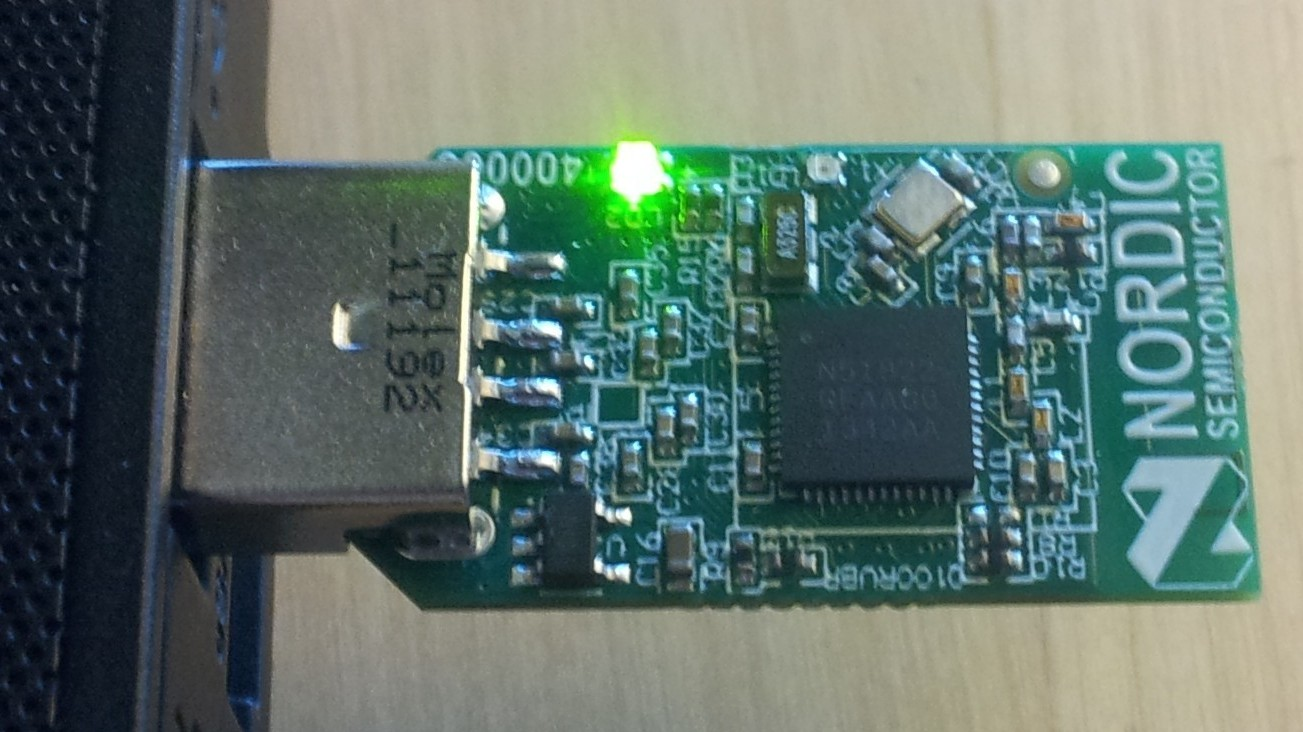
\includegraphics[width=\textwidth]{PCA10000}
\caption{PCA10000 development board}
\label{pca10000}
\end{figure} 

Nordic Semiconductor provides \gls{ble} stack as a precompiled and linked binary file called \emph{SoftDevice}. There are various of these SoftDevice binaries with different aspects of the \gls{ble} stack. The SoftDevice is stored in a protected area in the flash memory and has access to a protected section of \gls{ram} memory, preventing unauthorized access by the application code. The SoftDevice can be accessed through a specified set of \gls{api} calls. These \glspl{api} are accessed by making a supervisor call to the processor causing a exception handler to run the SoftDevice. All calls are non-blocking, which means that the call will not stall the application making the call. And there are synchronous and non-synchronous calls, where the synchronous calls immediately return the result while the asynchronous calls start an operation that will send the result as an event to the application. The SoftDevice is used for accessing the \gls{ble} stack as it was out of the scope of this thesis project to implement a \gls{ble} stack from scratch.

A \gls{sdk} is provided for nrf51822 which contains the peripheral drivers, application examples, the interface header files for the SoftDevices and their documentation. Two tools provided by Nordic Semiconductor has been extensively used in this thesis. \emph{nRF Sniffer} is a tool used with the PCA10000 board and \emph{Wireshark} application to capture, view and save the information of \gls{ble} packets being sent between two devices. This greatly helps in learning about \gls{ble} packets and debugging problems. This tool is capable of providing detailed information about almost all the segments of the captured packets. It was found in during the thesis project that the nRF-Sniffer is not entirely capable of capture each and every packet being communicated, which does limit its use as tool to get feedback as one develops low level \gls{ble} drivers. Another invaluable tool provided by Nordic Semiconductor is \emph{Master Control Panel}. It is an Android application which acts a generic \gls{ble} application capable of discovering \gls{ble} devices, connect and communicate with them while providing an overview of their Attribute database. 

%From actively using this platform for many months, the subjective pros and cons of this platform are stated below.
%
%\noindent Pros:
%\begin{easylist}[itemize]
%& Large, mature and active community
%& Support of open-source Eclipse and GNU-GCC development environment 
%& Availability at low price
%& Cortex M0 processor with competitive specs
%& Support in mbed, an online open source development platform
%& Support of supplementary tools such as nRF-Sniffer and android application 'Master Control Panel'
%\end{easylist}
%\vspace{5 pt} \noindent Cons:
%\begin{easylist}[itemize]
%& The \gls{ble} stack available as binary reducing flexibility
%& \gls{sdk} not open for distribution
%\end{easylist}

\section[Porting PCA10000 Platform of nrf51822 to Contiki]{Porting PCA10000 Platform of nrf51822 to Contiki\footnote{Available at \url{https://github.com/EarthLord/contiki} with complete Doxygen documentation}} \label{5Porting}

This section describes the process of porting Contiki to a new platform, specifically the nrf51822 based PCA10000. The development setup is described in section \ref{DevSetup} and the implementation of the peripheral drivers is described in section \ref{peripheralsContiki}. Additional information of the folder and makefile structure of Contiki can be found in section \ref{ApdxFolder} and \ref{ApdxMakefile} in Appendix \ref{ApdxContiki}

\subsection{Development Setup} \label{DevSetup}
Contiki was initially developed in a Linux based operating system, although Windows is also supported now. The porting of PCA10000 platform to Contiki was done in Ubuntu 13.10 and 14.04. The compiler suite used is GNU Tools for ARM Embedded Processors Version 4.8.3. The program used for programming the binary files compiled was SEGGER J-Link Commander V4.90 using the Segger JLink programmer on PCA10000. The front end used to write the code is the Eclipse IDE for C/C++ Developers Version Kepler Service Release 1 and Sublime Text. The porting was done to Contiki version 3.x, which is under active development.

\subsection{Peripherals required for Contiki}\label{peripheralsContiki}
This section details the implementation of the peripheral drivers done in this thesis so that the peripherals can be controlled with \glspl{api} specified by Contiki.
\paragraph{Contiki clock}
Contiki clock, which is the source for all the timers, except the rtimer, is provided by the RTC1 peripheral of nrf51822. RTC1 is chosen because when a SoftDevice is used, RTC0 will not be accessible for the user application. The \gls{rtc} peripheral uses the \gls{lfclk} of nrf51822, which can be generated by a crystal or RC oscillator to produce 32.768 kHz. For Contiki clock, in this thesis there are two driver implementations made, namely Tickless and Ticks as described below.

\subparagraph{Ticks}
For this implementation the RTC1 peripheral is configured such that an interrupt is called for its every increment or \emph{tick}, hence the name. This happens at 64 Hz, which is the default value of \texttt{CLOCK\_SECOND}. In the interrupt routine, the current clock tick is incremented, an etimer poll is requested if an etimer has expired and every \texttt{CLOCK\_SECOND}\textsuperscript{th} interrupt the second count is incremented. The variable storing the clock `ticks' and `seconds' is returned upon their request from any other process.

\subparagraph{Tickless}
In this implementation, the processor will not be woken up at every tick of the \gls{rtc} peripheral, hence the name. To enable this, a small addition is required to the etimer and clock module present at \texttt{CONTIKI/core/sys}. Every time the next etimer expiration is computed, the clock module is informed of it. With this additional information the \gls{rtc} can configure a compare interrupt to poll the etimer upon its expiry. The RTC1 peripheral is also configured to provide an interrupt only on its overflow so that it can be accounted for when calculating the seconds elapsed. For the 24-bit timer of RTC1, with \texttt{CLOCK\_SECOND} as 64, the overflow interrupt would happen only once every $(2^{24}/64)$ second, that is almost every three days. Compared to interrupt happening few times a second in the `Ticks' case this is a long time without the need for processor's involvement. With a Tickless implementation, both keeping track of the value of `clock ticks' and polling the etimer upon its expiry is handled by the \gls{rtc} peripheral rather than the processor, which would significantly reduce the power consumption without sacrificing any performance. Since changes need to be made to core Contiki library as mentioned above, this implementation is not supported natively by Contiki.

\paragraph{Rtimer}
An rtimer is implemented in Contiki's port to nrf51822 by using the \emph{TIMER1} peripheral, which runs on the \gls{hfclk} of 16 MHz. TIMER1 was chosen as TIMER0 is required by SoftDevice, in case it is used. Since rtimer is required with higher granularity than Contiki Clock, rtimer increments at rate of 62.5 kHz in its current implementation, which is every 16 \si{\micro \second}. This is achieved by TIMER1 being configured as a 8-bit timer and providing an interrupt on overflow where the rtimer count is incremented. In the interrupt routine there is also a check to see if the scheduled rtimer task needs to be run by comparing the current rtimer count. It should be noted that Rtimer being run by TIMER1 peripheral requires the \gls{hfclk} to be active, thereby consuming additional power.

\paragraph{\glspl{led}} 
The PCA10000 board has a RGB \gls{led} unit on it. The port allows it to be controlled by the Contiki \gls{api}. This is done through reading and writing to the \gls{gpio} port when the \gls{led}'s status is read and \gls{led}'s state is changed respectively. This implementation is present in `platform' folder since they are a property of PCA10000.
%\texttt{CONTIKI/platform/dev/led-arch.c}
%file since the \glspl{led} are not a property of the nrf51822 \gls{soc} but the PCA10000 platform.

\paragraph{Button(s)}
The PCA10000 board does not have any buttons. In case of porting a platform with physical buttons, its implementation would also be in the platform folder.

\paragraph{Serial Port}
The port of Contiki to PCA10000 platform offers abstraction of the \gls{uart} peripheral of nrf51822, which will communicate with the serial port of the computer to which PCA10000 is connected to. Writing to the serial port is achieved by using the \texttt{printf()} function present in the \texttt{stdio.h} library by redirecting \texttt{printf} call's character stream to the \gls{uart} peripheral. Instead of the default NewLib library, the Newlib-nano library is used so that the amount of memory required is reduced.

For receiving the data from the \emph{serial-line} module of Contiki is used. This module broadcasts an event when a series of characters are received ending with a `newline' (\textbackslash n) character. To use this module, it is initialized on boot and all the characters received by the \gls{uart} port is sent to this module in the \gls{uart} receive interrupt routine.

\paragraph{Radio} 

Since the radio peripheral is completely controlled by the SoftDevice for implementing the \gls{ble} stack, it is untouched in this port. To use the radio peripheral, the \glspl{api} provided by the SoftDevice is used. To see the work done in this thesis regarding the radio peripheral, refer section \ref{8AdvLogger}.

\chapter{Test Cases}

\section{Performance Metrics Definition}

\paragraph{Data Rate}

\paragraph{Latency}

\paragraph{Reliability}

\paragraph{Energy Consumption}

\section{Data Dump Test Design}

\begin{figure}[h]
    \centering
    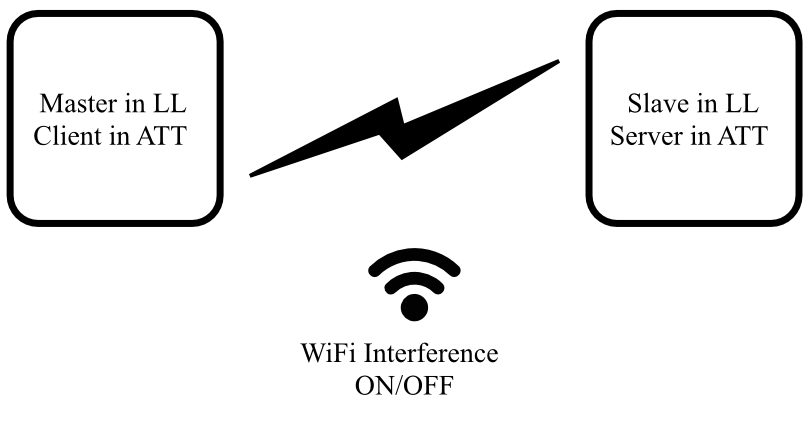
\includegraphics[width=\textwidth]{DataRateSetup}
	\caption{Setup to measure data rate with \gls{ble}}
    \label{fig:DataRateSetup}
\end{figure}

\begin{easylist}[itemize]
& Send packets of maximum size for one minute in the fastest way possible
&& Do one test without CCA for 802.15.4
& Repeat with WiFi
&& Choose a channel interfered by WiFi for 802.15.4 and one channel without WiFi interference.
&& For \gls{ble} do this with channel map with all channels and channel map with WiFi free channels.
& Do this test 10 times
\end{easylist}
\vspace{10pt}


In this test, to measure the various performance criteria in an environment with interference, WiFi interference will be introduced using the tool 'iperf'. The interference pattern generated will simulate streaming of large data over WiFi. \todo{Explain the exact configuration of UDP packets sent}

\vspace{10pt}
Metrics evaluated
\begin{easylist}[itemize]
& Data Rate
& Reliability
& Energy Consumption
\end{easylist}

\section{Request Response Test Design}

\begin{easylist}[itemize]
& Explain what is meant by request response
& Different cases in \gls{ble} and 802.15.4
\end{easylist}

Metrics evaluated
\begin{easylist}[itemize]
& Latency
& Energy Consumption
\end{easylist}


\pagebreak

The objectives of the tests are to compare the link layer of \gls{ble} and 802.15.4 in the aspects mentioned in the following sections. 

The \gls{ll} of 802.15.4 consists of \gls{mac} layer on top of a \gls{rdc} layer. For the RDC layer the Null-RDC and ContikiMAC driver will be tested in each of the test with \gls{csma} as the \gls{mac} layer. In case of Contiki-MAC the receiving node switches on periodically to sense if there are any packets that need to be received. The default time of this period is 125 ms. In case of null-RDC the radio receiver is never switched off, as the name suggests.

For \gls{ble}, communication will be done at the Generic Attribute (GATT) layer because the binary from Nordic Semiconductor used in this project does not provide APIs to access the lower layers in both peripheral and central devices. In all the tests the packet structure in 802.15.4 will be same as in \gls{ble} above the link layer.
In this test, to measure the various performance criteria in an environment with interference, WiFi interference will be introduced using the tool 'iperf'. The interference pattern generated will simulate streaming of large data over WiFi. \todo{Explain the exact configuration of UDP packets sent}
In \gls{ble}, the devices can assume different roles in the different layers of the protocol. In the \gls{ll} a device can be a 'Master' or a 'Slave'. In the \gls{att} layer, a device can be a 'Client' and/or 'Server'. A server contains data and the client can request data from the server.

In some of the tests, to measure the various performance criteria in an environment with interference, WiFi interference will be introduced using the tool 'iperf'. The interference pattern generated will simulate streaming of large data over WiFi.

\section{Data Rate Test}
This experiment aims to measure the maximum data rate of \gls{ble} and 802.15.4 at the LL with and without WiFi interference. For the \gls{ble} test the devices are configured as shown in the diagram below.

\begin{figure}[h]
    \centering
    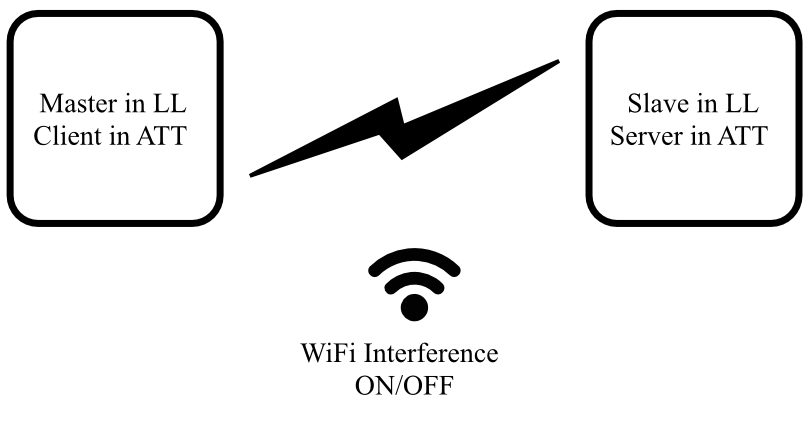
\includegraphics[width=\textwidth]{DataRateSetup}
	\caption{Setup to measure data rate with \gls{ble}}
    %\label{fig:DataRateSetup}
\end{figure}

In this test the data rate is measured by sending data from the server to the client which is not acknowledged in the \gls{att} layer. The data rate is measured at the receiver i.e the Master device. The packet structure will be used such that the complete packet size of \gls{ble} is used. Each run of the test will last of one minute to collect enough data to measure the average data rate.

In case of 802.15.4 one node is configured as transmitter and the other as receiver. The data-rate will be measured at the receiver. In these tests two channels will be used, one which interferes with WiFi and one which does not. This means that each channel will be tested with and without interference. The complete packet size of 802.15.4 will be used when conducting this test.

For data rate measurement tests in both the standards with and without WiFi, the data rate will be measured by sending data for one minute. The data rate will be expressed in both packets per second and \gls{kbps}. 

\subsection{Latency}
This experiment aims to measure the latency for a read request in case of \gls{ble} and 802.15.4, i.e. the time difference between sending the read request packet and receiving the packet with the value requested. In case of both the protocols there are intervals at which the radio is active, where communication can take place. To make sure that the read request packets are sent randomly at any point in this interval, timers with random values would be used to initiate sending these packets. The table below shows the connection parameters used for the various tests to measure the latency with \gls{ble}. The latency is measured at the device sending the packet '1' in the 'Packet' column and is defined as the time from sending the packet '1' to receiving the packet '2'.

\todo{Redo the correct table}


\begin{table}[htbp]
\begin{center}
\begin{tabular}{|l|l|l|l|l|}
\hline
\multicolumn{ 1}{|c|}{\textbf{Connection}} & \multicolumn{ 1}{c|}{\textbf{Connection}} & \multicolumn{ 3}{c|}{\textbf{Devices' Configuration}} \\ \cline{ 3- 5}
\multicolumn{ 1}{|c|}{\textbf{Interval}} & \multicolumn{ 1}{c|}{\textbf{Configuration}} & \multicolumn{ 1}{c}{\textbf{LL}} & \multicolumn{ 1}{|c}{\textbf{GATT}} & \multicolumn{ 1}{|c|}{\textbf{Packet}} \\ \hline
\multicolumn{ 1}{|c|}{} & \multicolumn{ 1}{l|}{Slave latency = 0} & Master & Client & 1. Read request \\ \cline{ 3- 5}
\multicolumn{ 1}{|l|}{} & \multicolumn{ 1}{l|}{
Supervision timeout = 1 \si{\second}} & Slave & Server & 2. Read response \\ \cline{ 2- 5}
\multicolumn{ 1}{|c|}{7.5 \si{\milli\second}} & \multicolumn{ 1}{l|}{Slave latency = 120
} & Master & Client & 1. Read request \\ \cline{ 3- 5}
\multicolumn{ 1}{|l|}{} & \multicolumn{ 1}{l|}{Supervision timeout = 1 \si{\second}} & Slave & Server & 2. Read response \\ \cline{ 2- 5}
\multicolumn{ 1}{|l|}{} & \multicolumn{ 1}{l|}{Slave latency = 120
} & Slave & Server & 1. Indication \\ \cline{ 3- 5}
\multicolumn{ 1}{|l|}{} & \multicolumn{ 1}{l|}{Supervision timeout = 1 \si{\second}} & Master & Client & 2. Indication ACK \\ \hline
\multicolumn{ 1}{|c|}{} & \multicolumn{ 1}{l|}{Slave latency = 0
} & Master & Client & 1. Read request \\ \cline{ 3- 5}
\multicolumn{ 1}{|l|}{} & \multicolumn{ 1}{l|}{Supervision timeout = 1 \si{\second}} & Slave & Server & 2. Read response \\ \cline{ 2- 5}
\multicolumn{ 1}{|c|}{125 \si{\milli\second}} & \multicolumn{ 1}{l|}{Slave latency = 15
} & Master & Client & 1. Read request \\ \cline{ 3- 5}
\multicolumn{ 1}{|l|}{} & \multicolumn{ 1}{l|}{Supervision timeout = 3 \si{\second}} & Slave & Server & 2. Read response \\ \cline{ 2- 5}
\multicolumn{ 1}{|l|}{} & \multicolumn{ 1}{l|}{Slave latency = 15
} & Slave & Server & 1. Indication \\ \cline{ 3- 5}
\multicolumn{ 1}{|l|}{} & \multicolumn{ 1}{l|}{Supervision timeout = 3 \si{\second}} & Master & Client & 2. Indication ACK \\ \hline
\end{tabular}
\end{center}
\caption{\gls{ble} latency measurement test cases}
\label{tbl:testcases}
\end{table}

Where,

\emph{Connection Interval}: After a \gls{ble} connection is established, the master device must always send a packet to the slave periodically after the time specified in connection interval. These connection events provide an opportunity for the slave to communicate with the master.

\emph{Slave Latency}: The maximum number of connection events that a slave can choose not to respond to the master. This is intended to save power on the slave while also providing an opportunity to communicate with the master if necessary.

\emph{Supervision Timeout}: A \gls{ble} connection is said to be lost if there is no bi-directional communication between the master and the slave for the duration specified by supervision timeout. After a tiemout the master will not send a packet to the slave in every connection event.

\emph{\gls{gatt} Read}: A packet containing an (attribute) value sent from a GATT server to a GATT client in response to a request from the client.

\emph{\gls{gatt} Indication}: A packet containing an (attribute) value sent from a GATT server to a GATT client, which the client should acknowledge (ACK). This packet is sent without the client requesting this data.

In the case of 802.15.4, one node is configured to send unicast messages and another is configured to receive these and send a response. The latency using both ContikiMAC and NullRDC will be measured. The latency is measured as the time difference between sending a unicast message and receiving its response.

The \gls{ble} test cases are designed such that the 7.5 \si{\milli\second} tests can compare with Null-RDC test of 802.15.4 while the 125 \si{\milli\second} tests can compare with the  ContikiMAC test of 802.15.4. There are tests with Slave Latency as zero and non-zero, which will help in identifying its effect on latency and the energy consumption of both the master and slave device.

To get an overall sense of the latency over a period of time, the average and standard deviation of the delay for 1000 transactions will be calculated for each test. In all the tests the payload will be of 20 bytes.

\subsection{Energy Consumption}
Energy consumption will be indirectly measured by logging the radio activity in all the tests described above in both the devices communicating. This will provide the duty cycle of when the radio is on. The possibility of logging the sleep cycle of the processor using the binary for \gls{ble} software needs to be verified. If the state of the processor is available, it will also be logged.

\subsection{Reliability}
Similar to measuring the energy consumption, reliability will be evaluated by  correlating the logs of when the radio is switched on versus when the packets are logged. This will provide an idea of how many times a packet has been dropped and hence find out the \gls{pdr}.

\chapter{Results and Analysis}

\section{Data Dump Test}

Add graph

\section{Request Response Test}

Add graph

\section{What we learnt}
\chapter{Other Contributions}

\section[Advertisement Logger]{Advertisement Logger\footnote{Available at \url{https://github.com/EarthLord/nrf51AdvLogger} with Doxygen documentation}} \label{8AdvLogger}

During the exploration phase of the thesis, the plan was to implement the required parts of the link layer of \gls{ble} from scratch. This included developing the entire radio driver. After looking into the radio peripheral of nrf51822 and working with it, this plan was abandoned due to lack of time to finish these tasks and the test cases. The work with the radio peripheral did result in developing a full-fledged BLE advertisement packet logger, whose interface (using CuteCom serial terminal) can be seen in figure \ref{fig:UIAdvLogger}. Detailed description can be found in Appendix \ref{ApdxAdvLog}. 

\begin{figure}[h]
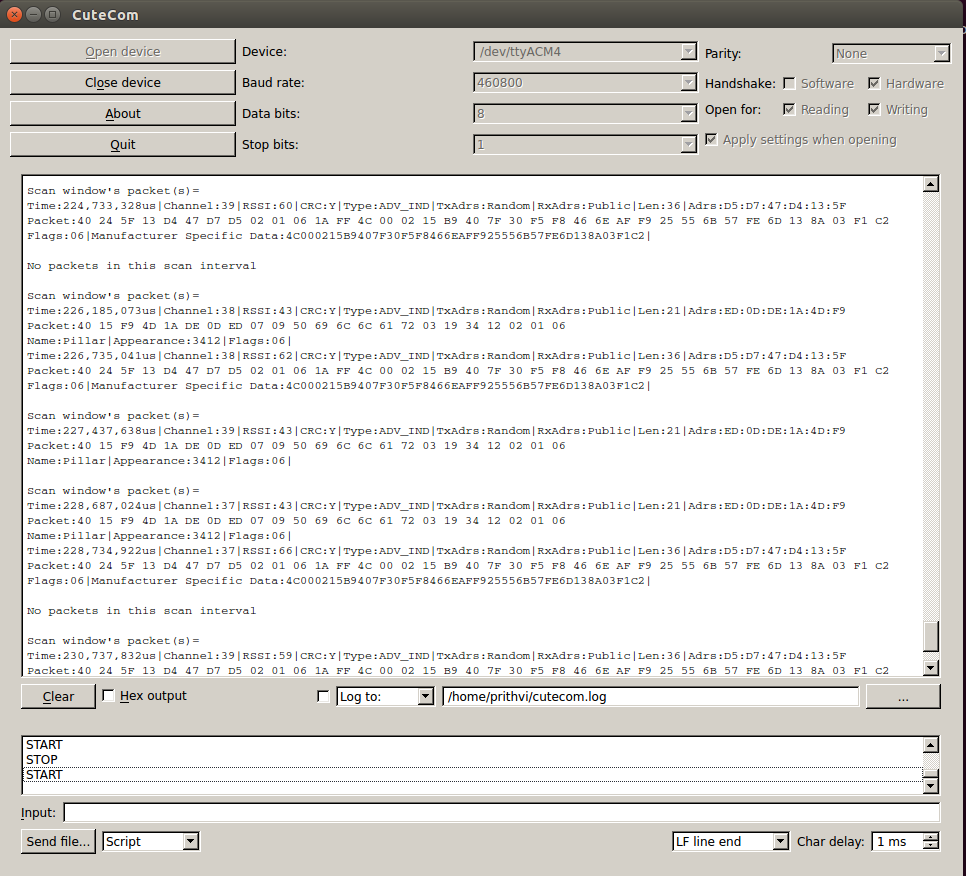
\includegraphics[width=0.97\textwidth]{AdvLogger}
\caption{User Interface of Advertisement Logger}
\label{fig:UIAdvLogger}
\end{figure}

\section[Firmware for an Alarm Device]{Firmware for an Alarm Device\footnote{Available at \url{https://github.com/EarthLord/contiki/tree/master/examples/PCA10000-nrf/Pillar}}}

A demonstration application was developed to test the port of Contiki on the nrf51822 platform. This application consisted of an alarm device controlled by a mobile application. The PCA10000 platform was used for this development too. The operations of setting of the next alarm time, canceling the alarm and also silencing the alarm can be done from a mobile application. The \emph{Master Control Panel} application by Nordic Semiconductor was used to test all the functionality.

The functioning of the alarm device with the mobile \emph{App} controlling it from a user's perspective can be seen in the state diagram in figure \ref{fig:AlarmAppDev}

\begin{figure}[h]
\centering
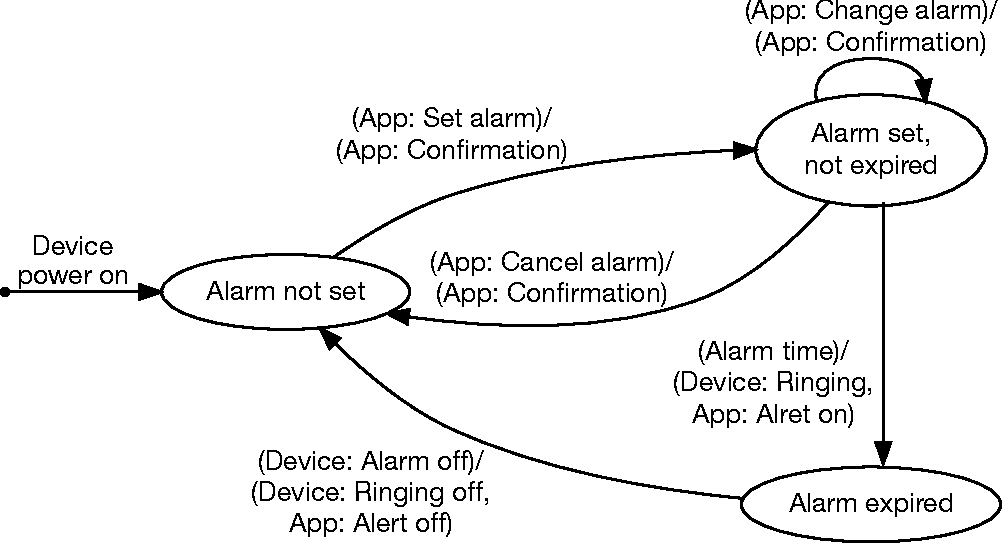
\includegraphics[width=0.9\textwidth]{AlarmAppDev}
\caption{State Diagram of an alarm device from an user's perspective}
\label{fig:AlarmAppDev}
\end{figure}

To achieve this a custom \emph{service} was created to contain two custom \emph{characteristics}. One characteristic contained the time to the next alarm and the other characteristic contained the status of whether the alarm is set or not, both with \gls{cccd}. The details of the two characteristics are:

\begin{tcolorbox}[sidebyside,colback=white,colframe=white]
\textbf{\underline{Next alarm time (§)}}
\begin{easylist}[itemize]
\ListProperties(Style1*=--)
\\• Read, write and notify allowed
\\• \gls{cccd} to disable/enable notifications
\\• Open link security mode
\\• No read/write authorization required
\\• 32-bit value
& 0 implies no alarm set
& Seconds to next alarm, if not 0
\end{easylist}\tcblower
\textbf{\underline{Alarm status (¶)}}
\begin{easylist}[itemize]
\ListProperties(Style1*=--)
\\• Read and notify allowed
\\• \gls{cccd} to disable/enable notifications
\\• Open link security mode
\\• No read/write authorization required
\\• 8-bit value
& 1 if alarm is set or ringing
& 0 if alarm is not set
\end{easylist}
\end{tcolorbox}


\begin{figure}[t!]
\centering
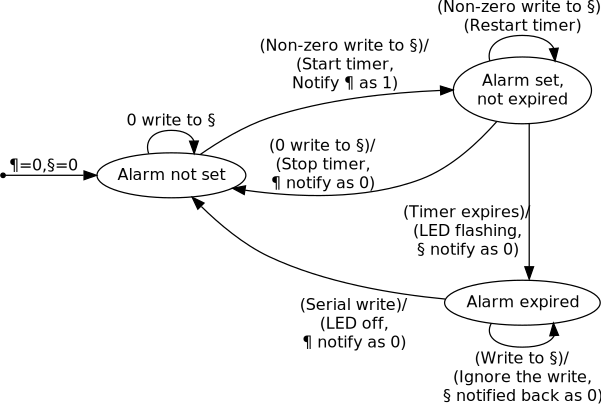
\includegraphics[width=\textwidth]{AlarmChar}
\caption{State Diagram of an alarm appcessory controlled by BLE}
\label{fig:AlarmChar}
\end{figure}

Apart from these characteristics, Contiki etimers and Contiki serial-line module from the Contiki port to nrf51822 are used for this alarm. Since the PCA10000 platform is used for this alarm device's development, the `ringing' of the alarm is done by flashing the \gls{led} on board and `silencing' the alarm is done by sending a string through the serial port. The state diagram in figure \ref{fig:AlarmChar} shows the implementation done for this alarm device. Note that (§) and (¶) represent the characteristics described above.

\chapter{Conclusion and Future Work} \label{9ConcFuture}
\section{Conclusion}

Contiki has been ported to a BLE based platform, namely the nrf51822 \gls{soc} based PCA10000 board. nrf51822 was chosen as the \gls{soc} to work with after comparing various commercially available \glspl{soc} based on the various requirements from the platform. The port allowed all the basic peripherals of nrf51822 to be controlled by Contiki's libraries such as etimer, rtimer, serial-line and LEDs.  The radio was not included in the port since the radio was controlled by a SoftDevice binary for BLE operations and also since the Contiki radio \glspl{api} are not compatible with BLE operations. The test cases and the alarm application developed with Contiki verified its working with this platform. Compatibility of Contiki with a BLE based platform provides an event based OS to be used for developing BLE applications.

Two test suites were designed to compare four metrics of the link layer of BLE and 802.15.4, where 802.15.4 refers to use of 802.15.4 physical layer and use of either ContikMAC and Null-RDC \gls{mac} layer as the \gls{mac} layer. The four metrics that were compared were data rate, reliability, latency and energy consumption. Two test suites were designed to collect data of these four metrics and compare the two protocols. Some test cases also included presence of external interference caused by presence of heavy WiFi traffic. The scenario assumed was where one device is unconstrained with respect to availability of power while the other is not.

This thesis shows that the data rate achievable with 802.15.4 is greater than BLE due to the larger packet size and having the radio on 100\% of the time, although BLE consumes lesser energy. In case of BLE the data rate highly depends on the software stack being used. The data rate achievable with BLE is suitable for application up to streaming of audio.  

In terms of reliability, the error detection and retransmission of data has shown that the upper layer in BLE can consider the link layer as completely reliable. The frequency hopping mechanism of BLE ensures that any narrow band interference in the 2.4 GHz ISM band does not break down the communication. If the channels used for frequency hopping is chosen adaptively then the interference will not have any effect on BLE communication. Unlike in BLE, 802.15.4 does have a back-off mechanism to prevent communication in case there is external interference. This thesis shows that this mechanism has greater efficiency when there is lesser interference. 

BLE has better minimum latency than 802.15.4 although ContikiMAC with 125 ms wake up interval has better latency than BLE with 125 ms connection interval. The latency with a BLE connection for a request response operation depends on two connection parameters, namely connection interval and slave latency. The energy consumption also depends on these two parameters. The advantage of BLE over 802.15.4 is the ability of changing the connection parameters on the fly. This will allow optimizing the connection according to changing requirement depending on external conditions. 

%The conclusion is that now BLE can be used with Contiki and gained better understanding of the technology.
%By comparing with 15.4 we see that it has a competitive advantage in reliability and run-time reconfigurability.
%Mention that we expect this work to enable more research and product development in low-power IoT with Bluetooth.

One of the major strengths of BLE is its standardization with Bluetooth 4.0 core specification which has enabled its inclusion in millions of consumer devices. This has made it the communication protocol of choice for all the accessory devices which require human to machine communication. The standardization allows devices from different manufacturers to communicate with each other without issues. On the other hand 802.15.4 protocol is not adopted in major consumer devices. There has been extensive research on protocols based on 802.15.4 physical layer which has resulted in many standards being developed. There is native support for mesh network in protocols based on 802.15.4 which allows applications such as home automation and smart grid. This makes protocols based on 802.14.5 preferable for applications that require machine to machine communication.

Overall this work is expected to enable further research and product development in low-power IoT with Bluetooth Low Energy.

%In terms of the data rate, the 802.15.4's NullRDC layer achieved the highest at 155 kbps without Clear Channel Assesment (CCA). The effect of WiFi interference overlapping in the channel of communication in case 802.15.4 can be seen when the data rate reduced to 61 kbps from 148 kbps in the case where interference was in a different channel. With 802.15.4 the data rate can be maximized by having Radio Duty Cycle (RDC) of 100\%. The influence of frequency hopping in BLE can be noticed when the data rate decreased to only 23 kbps from 29 kbps when WiFi interference was introduced, both cases having RDC of around 27\%.  In BLE the effect of packets communicated per connection interval can be seen when communicating with an Android device as the data rate increased to 86 kbps, in which RDC was 44\%. 
%
%Use of 802.15.4's CCA delivered a Packet Reception Ratio (PRR) of 99\% and 79\% with and without WiFi interference respectively. In case of BLE, the link layer's the simple acknowledgment scheme achieved a Packet Delivery Ratio (PDR) of 100\%. Without WiFi interference, BLE achieved a PRR of almost 100\%. When WiFi interference was introduced, PRR resurged back to greater than 99\% when WiFi free channel map was used as compared to 80\% when complete channel map, which shows working of Adaptive Frequency Hopping (AFH).
%
%802.15.4's latency was measured as 24 ms with Null-RDC and 90 ms with ContikiMAC. With BLE latency values ranging from 14 ms to 750 ms were observed. These tests to measure latency show the influence of link layer parameters such as `connection interval' and `slave latency', as well as whether the data is queried by the master node or the slave node. The change in symmetry of the connection with non-zero slave latency can be seen in case where the latency changes from 16 ms to 736 ms when the test case changes from the slave querying the data to the master querying the data. The master's RDC of 22\% and slave's RDC of 0.6\% also indicates the asymmetry in the connection. With these different configurations, the different use cases are also illustrated.

%
%\begin{easylist}[itemize]
%& The absolute data rate achievable with 802.15.4 is higher than BLE on the account of the greater link-layer payload size, which is 110 byte for 802.15.4 and 27 byte for BLE. This is even with BLE having higher bit rate (1 Mbps) compared to 802.15.4 (250 kbps).
%& The highest data rate achieved with 802.15.4 is when \gls{cca} wasn't used (155 kbps), followed by communicating with a channel not overlapping with external interference using \gls{cca} (148 kbps).
%& When WiFi interference was present in the channel used, the lack of \gls{cca} resulted in higher data (114 kbps) rate as compared to \gls{cca} enabled (61 kbps).
%& In case of BLE, the highest data rate was recorded when communicating with an Android device (86 kbps), since the master device allowed multiple packets to be communicated in a connection interval. 
%& The data rate achieved between PCA10000 nodes was in-line with the theoretically calculated data rate when there was no external interference (29 kbps). This is the same case when WiFi free channel map was used with external interference. Since this is as if \gls{afh} is implemented, there is no degradation in the data rate. When there was WiFi interference and the complete channel map was used, the data rate dropped to only 80\% of the interference free data rate because of the frequency hopping.
%& The data rate achieved in BLE communication depends highly on the stack, which limits the deciding parameters of connection interval and packets communicated consistently in each connection interval.
%& \gls{cca} operation in 802.15.4 has greater efficiency in case of low external interference (99\% \gls{prr}) as compared to high external interference  (79\% \gls{prr}).
%& The acknowledgment scheme of BLE does result in 100\% \gls{pdr} for the layers above the link layer in all cases. The \gls{prr} with BLE is greater than 99\% when there was no external interference and when WiFi free channel map was used. 80\% \gls{prr} was achieved when all the channel map was used with external interference, which shows that narrow band interference affects only a small portion of the communication.
%& When one packet was communicated per connection interval, the \gls{rdc} was between 26 and 29\%. This value increased to about 44\% when an average of 3 packets were communicated per connection event.
%& Null-RDC with radio on always achieved least latency for 802.15.4 for a read-response operation with a mean delay of 24 ms. When the more practical ContikiMAC layer was used the mean delay increased to 90 ms, but with the responding node only having its radio on for 1.3\% of the time.
%& The latency measurement with BLE nodes ranged from 14 ms to 750 ms depending on the configuration. One directly contributing factor is the connection interval used. With a greater connection interval the latency also increased.
%& By using non-zero slave latency the slave node's energy consumption decreased and the effect on latency measurement was dependent on which node initiated the request for data. When the master node initiated the request for data the latency increased but when the slave node initiated the communication the latency was as in the case with zero slave latency. 
%& This ability of BLE to create asymmetric connection  can illustrated in the case where the slave device's energy consumption drops drastically without change in the latency when using indication packets. This can result in cases where 14 ms latency can be achieved by a master and slave node consuming only 21.5\% and 0.54\% radio on time.
%& Use cases where low latency is required for data to communicated from the master to slave, the slave latency value used must be close to zero. In other cases large slave latency values can be used. The provision for dynamic update of the link layer parameters of a BLE connection is useful in optimizing these parameters for different scenarios.
%
%\end{easylist}

\section{Future Work}

This project's experiments conducted only a subset of possible configurations with which both BLE and 802.15.4 could be used, although an overview has been provided. Various other configurations in terms of variation of the power constraint on the nodes, test case configuration and connection parameters can be used to gain better insight and comparison between BLE and 802.15.4.

The lack of availability of a complete and open-source BLE stack is one of the major inhibiting factors faced by researchers working with \gls{ble}. This results in little or no flexibility in developing the test setup as needed for the research projects. Contiki is a mature platform under active development for \gls{iot} projects. This thesis project can provide a start to active development of an open-source BLE stack and support for greater number of BLE based platforms in Contiki.

Bluetooth \gls{sig} has released the Bluetooth 4.1 Core Specification in December 2013, which provides numerous improvements to the existing features while adding support to various new features \cite{4.1ExtendsIoT}. This evolutionary update to Bluetooth lays the foundation to include IP based communication in the future updates \cite{4.0to4.1}. The organization Internet Engineering Task Force (IETF) has a working draft of the standard for communicating over IPv6 over BLE \cite{ieftIPv6Draft}, taking into account the Bluetooth 4.1 specification. This draft includes the addition of support for 6LowPAN over BLE. All these developments make it important to adopt these specifications to be compatible with the future devices and work on IPv6 communication over BLE. 

One of the major constraints of the BLE protocol is the lack of support for multi-hop networks. This has lead to the majority of usage in applications with human to machine communication. Enabling IPv6 communication and multi-hop network with BLE enables a host of additional applications in the \gls{iot} domain, just as BLE started the \emph{appcessories} market.

\chapter{Appendix | Advertisement Logger's Implementation} \label{ApdxAdvLog}

\section{Scanning \gls{ble} Advertisements}

According to the Bluetooth 4.0 Core specifications, an advertisement event consists of an advertising device periodically send advertisement packets. The interval of these advertising events can range from 20 ms to 10 s. In each of these advertising events an advertiser sends an advertising packet in each channel in an interval of 10 ms starting with channel 37. The objective of a BLE advertisement scanner would be to be able to receive the packets from at least one channel in an advertisement event, while saving power. To achieve this trade off, the radio duty cycles between receiving and disabled state, while being in the next advertising channel every time it is switched on. The total time of this periodic event is known as the \emph{Scan Interval}, while the time the radio is on is known as \emph{Scan Window}. The figure\footnote{\href{https://devzone.nordicsemi.com/question/2535/what-is-the-minimum-time-for-a-app-and-a-peripheral-to-create-a-connection/}{https://devzone.nordicsemi.com/question/2535/what-is-the-minimum-time-for-a-app-and-a-peripheral-to-create-a-connection/}} \ref{fig:AdvScanBLE} depicts this process.

\begin{figure}[h]
\centering
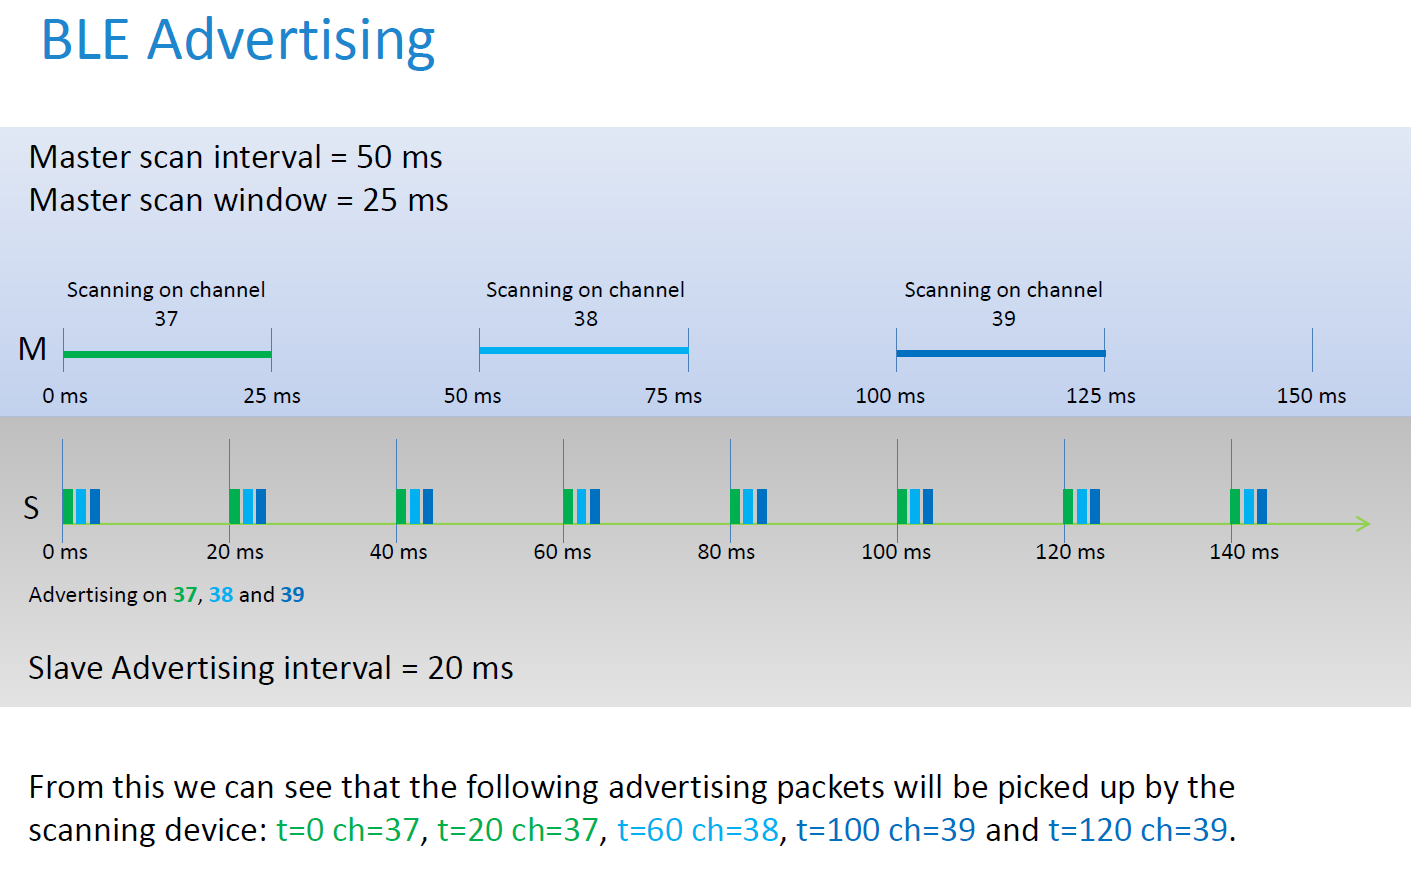
\includegraphics[width=\textwidth]{AdvScanBLE}
\caption{Scanning BLE advertisements}
\label{fig:AdvScanBLE}
\end{figure}

\section{Software Architecture}
The following flow charts explain the software architecture of the \emph{Advertisement Logger}.
\subsection{Main Function}
The execution of the program starts with the main function after reset as depicted by figure \ref{fig:main_chart}. Note that the radio is initialized to continuously receive packets once it has started while also measuring the received signal strength \acrshort{rssi}.
\begin{figure}[h]
\centering
\vspace{80pt}
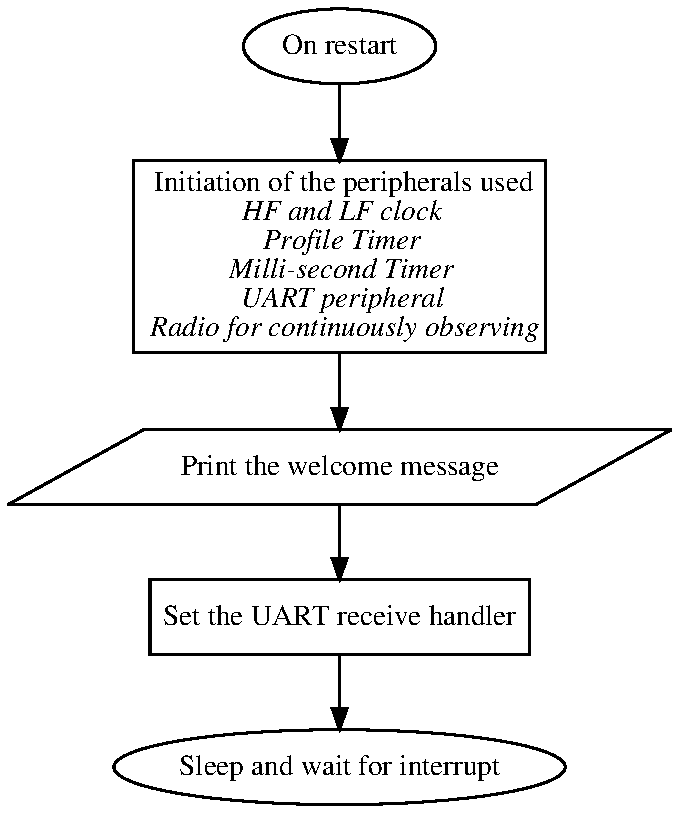
\includegraphics[scale=0.85]{main_chart}
\caption{Main function flowchart}
\vspace{80pt}
\label{fig:main_chart}
\end{figure}

\subsection{UART String Receive Handler}
The UART String Receive handler which gets a string sent to the \gls{soc} through an unsigned character pointer checks if the string is either \texttt{START} or \texttt{STOP} so that the scanning of the advertisements can be started or stopped respectively.
\begin{figure}[h]
\centering
\vspace{50pt}
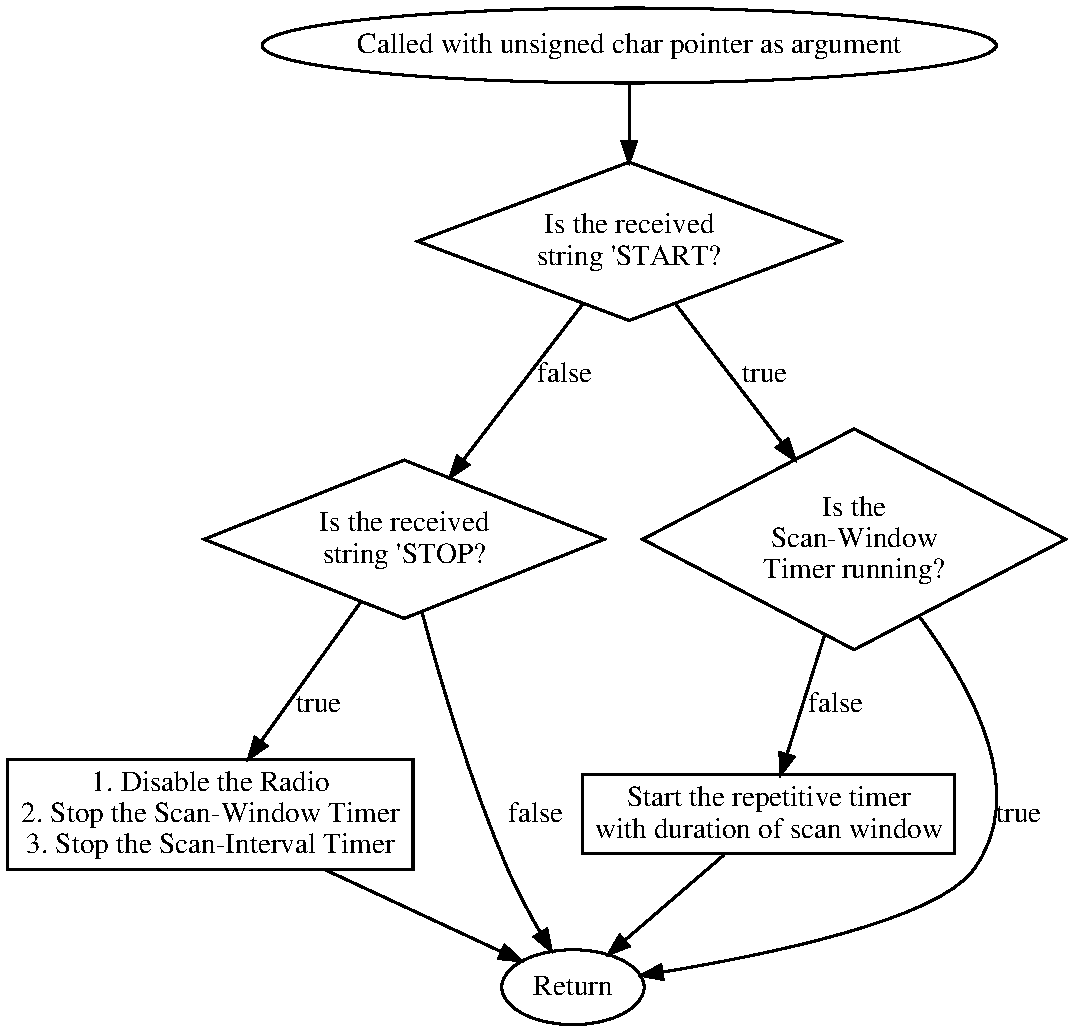
\includegraphics[scale=0.85]{UartISR_chart}
\caption{UART string receive handler flowchart}
\vspace{51pt}
\label{fig:UartISR_chart}
\end{figure}
\clearpage

\subsection{Scan Interval Timer Handler}
The scan interval timer is a repetitive timer with an interval equal to the scan interval. At the beginning of the scan interval this function performs 5 different tasks as shown in figure \ref{fig:scanInterval_chart}.
\begin{figure}[h]
\centering
\vspace{20pt}
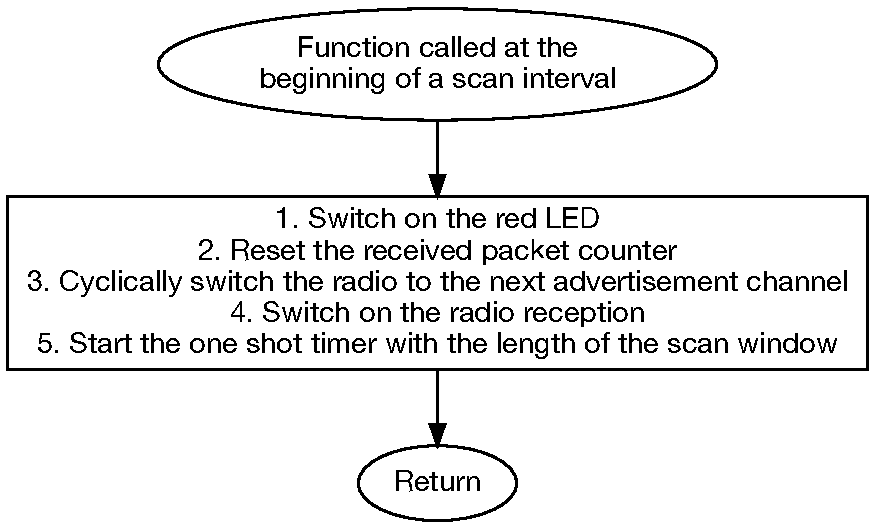
\includegraphics[scale=0.85]{scanInterval_chart}
\caption{Scan interval timer handler flowchart}
\label{fig:scanInterval_chart}
\end{figure}

\subsection{Scan Window Timer Handler}
The scan window timer is a single shot timer with an interval equal to the scan window. At the end of the scan window this function performs 3 different tasks as shown \ref{fig:scanWindow_chart}.
\begin{figure}[h]
\centering
\vspace{20pt}
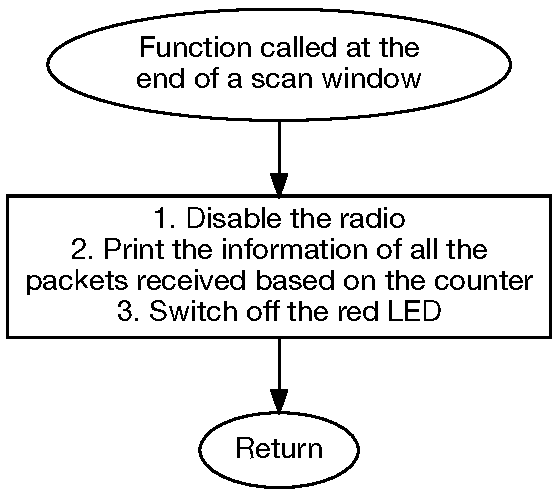
\includegraphics[scale=0.85]{scanWindow_chart}
\caption{Scan window timer handler flowchart}
\label{fig:scanWindow_chart}
\end{figure}

\subsection{Radio Interrupt Routine}
The radio peripheral is configured such that the end of a packet and the end of \acrshort{rssi} measurement trigger the interrupt. At the end of a packet, the packet's data is collected if there is space in the buffer. At the end of the \acrshort{rssi} measurement the \acrshort{rssi} value is saved.
\begin{figure}[h]
\centering
\vspace{10pt}
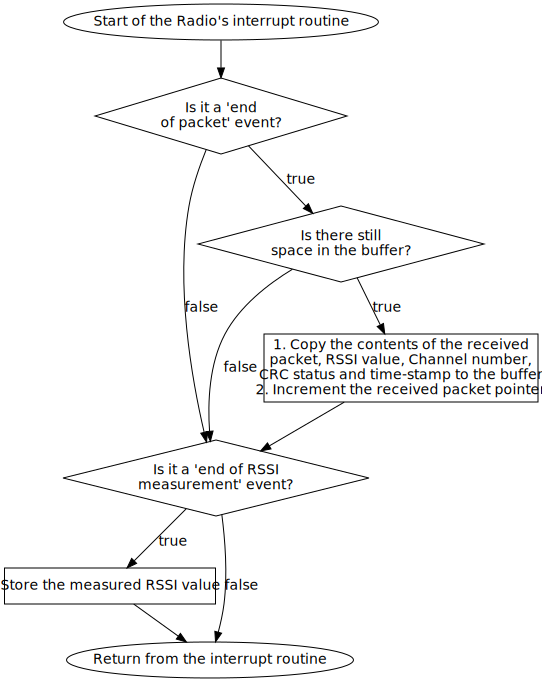
\includegraphics[scale=0.85]{RadioISR_chart}
\caption{Radio interrupt routine flowchart}
\label{fig:RadioISR_chart}
\end{figure}

\chapter{Appendix | \gls{ble} \gls{soc} Comparison} \label{ApdxSoC}
The dense table in the next page compares many different parameters of the \gls{ble} \glspl{soc} available. This table was compiled in the first half of 2014. Because of the high pace at which the industry around \gls{ble} is progressing, many details here might not be accurate as time progresses.

The legend for the table is

\vspace{10pt}
NA \hspace{10pt}: The information is not available

- \hspace{22pt}: The feature is not available

\includepdf[pagecommand={\begin{tikzpicture} [remember picture,overlay] \node at (7.4,-17) {}; \end{tikzpicture}}]{BLE_SoCs.pdf}

\chapter{Appendix | Data Acquired} \label{ApdxData}

The entire data acquired and results computed for both High-Throughput test and Request-Response test can be found in the tables in the following pages.

%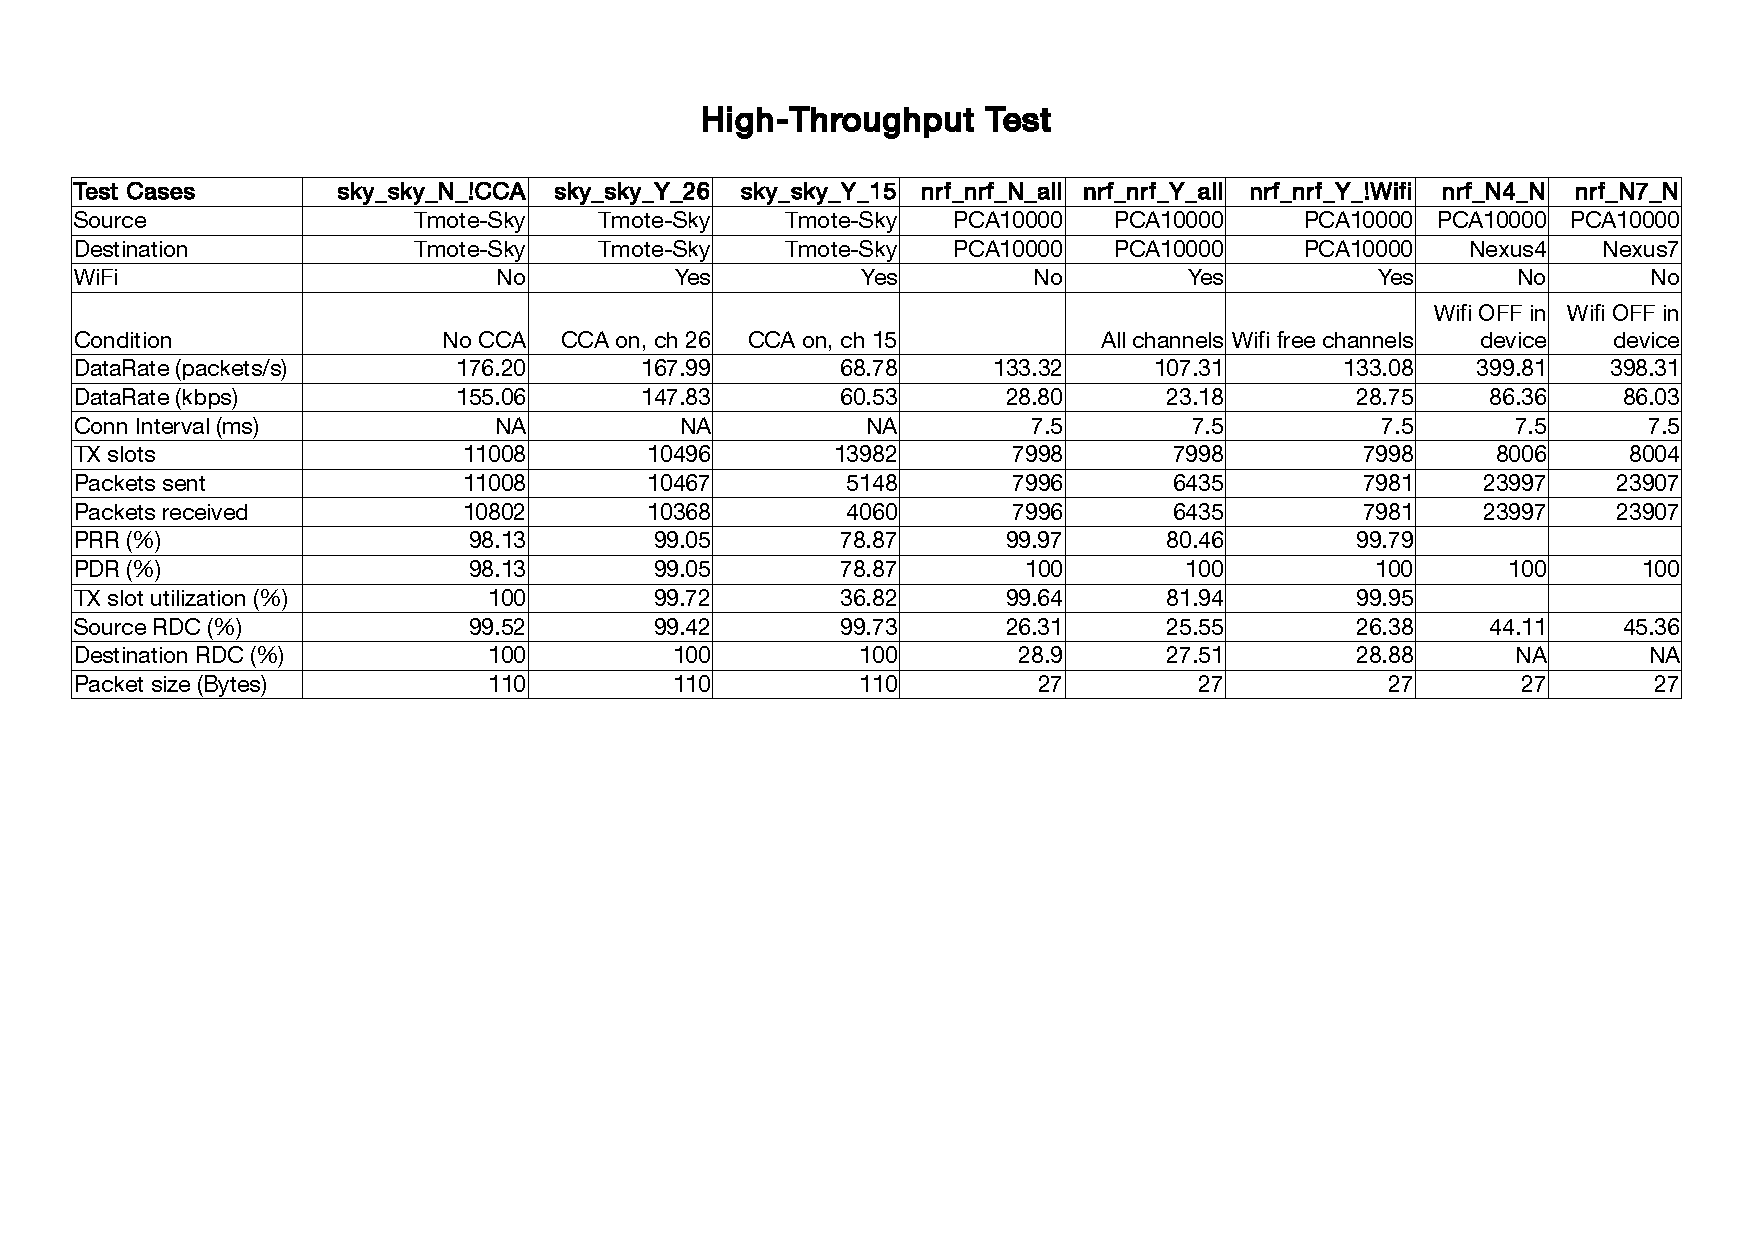
\includepdf[landscape]{HT.pdf}
%
%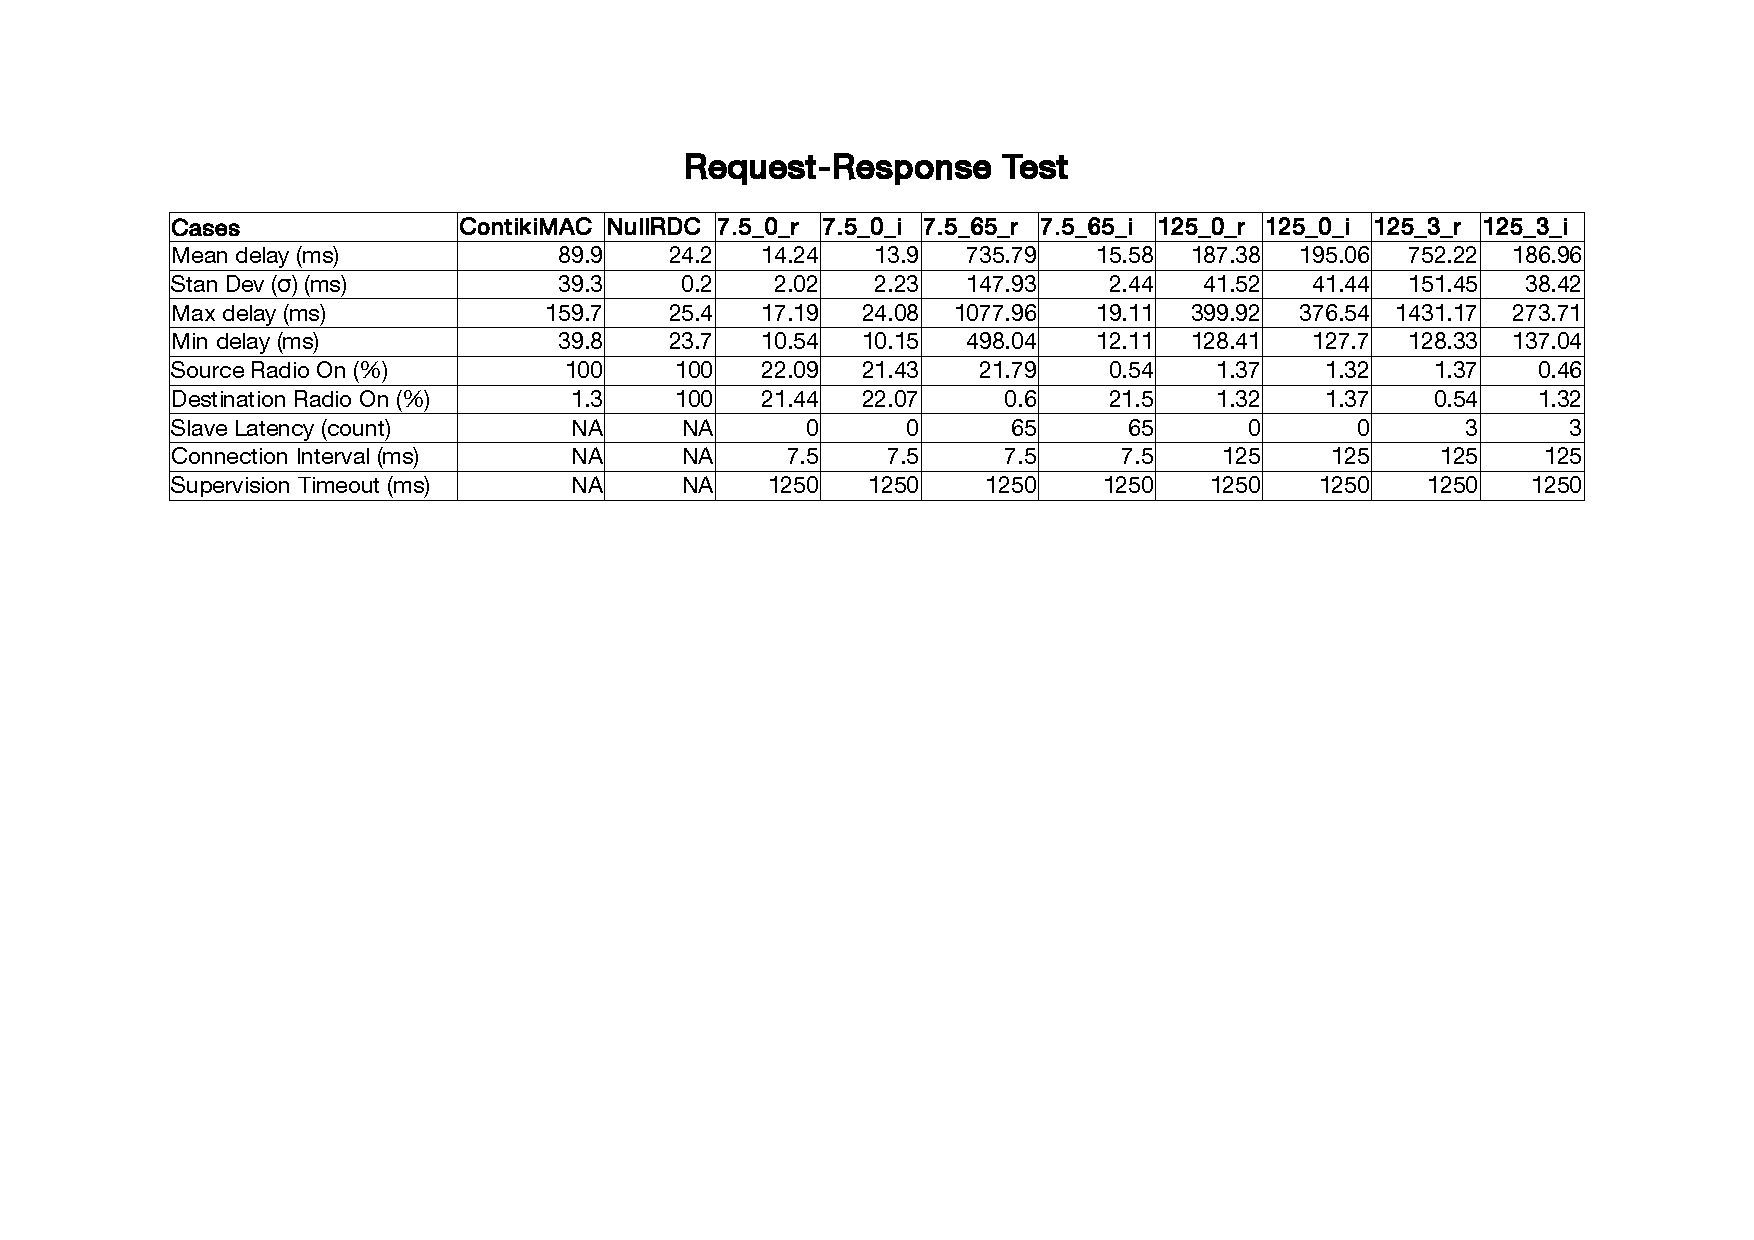
\includepdf[landscape]{RR.pdf}

\printbibliography[title={References}]

\end{document}          
